\documentclass[oneside]{book}
%\documentclass[openany]{book}
%\documentclass{book}

\usepackage{graphicx}

\usepackage{amsmath}
\usepackage{mathtools}
\usepackage{amssymb}
\usepackage{comment}

\usepackage{amsthm}
\usepackage{mathrsfs}
\usepackage[T1]{fontenc}
%\usepackage{libertine}
\usepackage[english]{babel}
\usepackage{lmodern}


\usepackage{hyperref}

\newtheorem{theorem}{Theorem}[section]
\newtheorem{corollary}{Corollary}[theorem]
\newtheorem{lemma}[theorem]{Lemma}
\newtheorem{mydef}{Definition}[section]
\newtheorem{exmp}{Example}
\newtheorem{prop}{Proposition}
\newtheorem{properties}{Properties}[section]
\date{\today}
\hypersetup{
	colorlinks=true, %true if colored links
	linktoc=all,     %all if both sections and subsections linked
	linkcolor=blue,  %color links
}
\usepackage[utf8]{inputenc}
\usepackage{csquotes}


\begin{document}
	
	\begin{titlepage}
		\begin{center}
			\vspace*{1cm}
			
			\Huge
			\textbf{Isoperimetric Inequality}
			
			\vspace{0.5cm}
			\LARGE
			
			
			\vspace{1.5cm}
			
			\textbf{Prashant Kumar}
			
			\vfill
			
			\textit{A dissertation submitted for the partial fulfilment of BS-MS dual degree in Science}          
			\vspace{0.9cm}
			
\includegraphics[width=0.4\textwidth]{iiser logo.png}		
			
			\Large
			Department of Mathematical Sciences\\
			Indian Institute of Science Education and Research Mohali\\
			India\\
			June 2020
			
		\end{center}
	\end{titlepage}
	
	
	
	
	\urlstyle{same}
	
	\tableofcontents
	
	
	\thispagestyle{empty}
	\addcontentsline{toc}{chapter}{Certificate of Examination}
	\pagenumbering{roman}
	\chapter*{Certificate of Examination}
	
	This is to certify that the dissertation titled \enquote{Isoperimetric Inequality} submitted by Prashant Kumar (Reg. number $-$ MS15114) for the partial fulfillment of BS-MS dual degree program of the Institute, has been examined by the thesis committee duly appointed by the Institute. The committee finds the work done by the candidate satisfactory and recommends that the report be accepted.\\\\
	\textbf{Dr. Soma Maity} (Supervisor)\\
	\\
	\textbf{Dr. Lingaraj Sahu}  \hfill           \textbf{ Dr. Pranab Sardar}\\
	\\
	\\
	\rightline{\textbf{Date:} June 2020}
	\thispagestyle{empty}
	\addcontentsline{toc}{chapter}{Declaration of Authorship}
	
	\chapter*{Declaration of Authorship}
	The work presented in this dissertation has been carried out Juneby me under the guidance of \textbf{Dr. Soma Maity} at the Indian Institute of Science Education and Research, Mohali.
	This work has not been submitted in part or in full for a degree, a diploma, or a fellow- ship to any other university or institute. Whenever contributions of others are involved, every effort is made to indicate this clearly, with due acknowledgement of collaborative research and discussions. This thesis is a bonafide record of original work done by me and all sources listed within have been detailed in the bibliography.\\
	\\
	\textbf{Prashant Kumar} (Candidate)\\
	Date: June 2020\\
	\\
	\\
	\\
	In my capacity as the supervisor of the candidate$'$s project work, I certify that the above statements by the candidate are true to the best of my knowledge.\\
	\\
	\textbf{Dr. Soma Maity}(Supervisor)\\
	Date: June 2020
	\thispagestyle{empty}
	\addcontentsline{toc}{chapter}{Acknowledgements}
	\chapter*{Acknowledgments}
	
	On this occasion, I would like to thank Dr Soma Maity, my Thesis supervisor, for giving me the opportunity to do this MS project on the fascinating topic of isoperimetric inequality. It is a golden opportunity for me. All through my ms thesis, she was a beacon of knowledge to me. 
	Her suggestions, outstanding guidance , support, passion and inspiration all through the project made me realize various topics and made me realize and understand the topic from a broader perspective. \\ 
	
	I would like to thank the members of my Thesis Committee: Dr Pranab Sardar and Dr Lingraj Sahu who not only empowered me but also recommended and provided valuable feedback on my thesis. \\
	
	I sincerely thank Neeraja Sahastrabudhe for proposing me additional related topic to my thesis "Isoperimetric Inequality for Graphs"  during her "Random Graph" course. \\
	
	Support and help from my elder brother Mr. Rajiv Krishna Omar on some doubts in part "Isoperimetric Inequality for Graphs" of my thesis and technical support during writing thesis in the home would not be forgotten.\\
	
	The scholarship granted for my MS curriculum by the Innovation in Science Pursuit for Inspired Research(INSPIRE) Scholarship of the Department of Science and Technology(DST), is duly acknowledged.\\
	
	
	I would like to thank IISER Mohali in particular, the Department of Mathematics, which provided me an amicable atmosphere to study various fields. \\
	
	Without the aid and love of all my intellectual peers who consistently \\supported and encouraged at IISER Mohali over the course of five years, there is really no way I could have done much. Nilangshu, Yogesh, Rajesh, Vidur, Adeeb, and Paresh are those buddies. 
	\\
	
	I am genuinely grateful to Dharm, Amit, Bhavya, Ajay, Ravinder, Shubham, Surendra, Ayush, Saurabh and Raj Kumar for their incredible company,
	support and guidence that enlightened my life in many different ways.\\
	
	I am forever grateful to my parents, grandparents and my brother and sister for always believing in me and for their continuous encouragement during my BS-MS journey.
	\thispagestyle{empty}
	
	\addcontentsline{toc}{chapter}{Abstract}
	\chapter*{Abstract}
	
	In this thesis, we first study Isoperimetric Inequality in $\mathbb{R}^{n}$ and then give some introduction to convex geometry and then get Isoperimetric inequality for convex bodies as a corollary followed by important theorem Brunn Minkowski theorem and its proof in convex geometry.
	
	
	
	
	
	
	
	
	
	
	
	
	
	
	
	
	
	
	
	
	
	
	
	
	
	
	
	
	
	
	
	
	
	
	
	
	
	
	
	\chapter{Introduction}
	\pagenumbering{arabic}
	\label{chap:c1}
	
	"Isoperimetric" means to have the same perimeter. Isoperimetric  inequality is a geometric inequality relating  the perimeter and volume of a domain. Classical Isopermetric inequality in the plane is that among all the closed curves of the fixed perimeter, which curve, if any, maximizes the enclosed area? Or otherwise, in the plane surrounding a fixed area, among all the closed curves, which curve minimizes the perimeter? \\
	
	Isoperimetric Inequalities are defined for various space like for Ecludian space and Reimannian manifolds. In ecludian space sharp Isoperimetric Inequality are found with equality while in Reimannian manifolds Isoperimetric Inequality are not exact but are close enough to get its global geometric information. Here We will be discussing only  Isoperimetric Inequality in Ecludian spaces e.g. in  $\mathbb{R}^{n}$ and then specifically in convex subsets of $\mathbb{R}^{n}$.
	\\
	\\
	In chapter 2 We first give some preliminaries in which some basic definitions and terms related to Convex Geometry are defined.In chapter 3, Isoperimetric Inequality in $\mathbb{R}^2$ is defined and formula is generalised for $\mathbb{R}^n$ and then discuss theorem which talks about uniqueness of existence of solution to Isoperimetric Problem which is disk and discuss proof of it using classical calculus. After that we discuss proof of Isoperimetric Inequality in $\mathbb{R}^2$  using 2-dimensional divergence theorem. \\
	Now we define Reimannian metric which is the first fundamental form and  riemannian divergence  along with second fundamental form and curvatures (Mean Curvature and Gauss-Kronekar Curvature) and then study Isoperimetric Inequality in domains with $\mathcal{C}^2 $ boundary and prove  results for first variation  of volume and area under a 1-parameter family of diffeomorphism.
	
	
	
	
	
	
	
	
	
	
	
	
	
	
	
	
	
	\chapter{Preliminaries }
	\label{chap:c2}
	
	
	
	
	
	
	
	
	
	
	
	
	
	
	
	
	\section{\textbf{Basic Definitions}}\label{s:1}
	\subsection{Curvature}
	\label{ss:1}
	
	For any $C^{2}$ path $\omega:(\alpha, \beta) \rightarrow \mathbb{R}^{2}$, Its derivative $w'$ is the velocity vector field  and the acceleration vector field is the second derivative  $w'$, assuming that w is an immersion (i.e. $ w' $ never vanishes) in the plane. Small infinitesimal element of the length of the arc is given $d s=\left|\omega^{\prime}(t)\right| d t$.
	\\Unit tangent vector field along $\omega$ is $\mathbf{T}(t)$ defined as \\
	
	\begin{equation}
	\label{eq1}  
	\textbf{{T}}(t)=\frac{\omega^{\prime}(t)}{\left|\omega^{\prime}(t)\right|}
	\end{equation}  \\
	and unit normal vector field $\mathbf{N}$ along $\omega$ is defined as 
	\begin{equation}
	\label{eq2}  
	\mathbf{N}=\mathbf{\tau} \mathbf{T}
	\end{equation} \\
	where $ \tau: \mathbf{R}^{2} \rightarrow \mathbf{R}^{2}$ is the rotation of $\mathbb{R}^{2}$ by $\pi / 2$ radians, and
	
	Then its curvature $\kappa$ is defined as
	\begin{equation}
	\label{eq3}  
	\frac{d \mathbf{T}}{d s}=\kappa \mathbf{N}
	\end{equation}  
	
	from equation (\ref{eq3} ) we have
	$$ \frac{d \mathbf{T}}{d s} \cdot \mathbf{N} = \kappa $$
	$\mathbf{N}$ and $\mathbf{T}$ are perpendicular to each other so that $\mathbf{N} \cdot \mathbf{T} = 0 $
	and on differentiating with respect to $s$ we get 
	$$ \mathbf{N} \cdot \frac{d \mathbf{T}}{d s} + \mathbf{T} \cdot \frac{d \mathbf{N}}{d s} = 0 $$ 
	so that we get
	\hfill \break  
	$$ \mathbf{T} \cdot \frac{d \mathbf{N}}{d s} = -  \mathbf{N} \cdot \frac{d \mathbf{T}}{d s} = -\kappa  $$ 
	and hence finally get 
	\begin{equation}
	\label{eq4}  
	\frac{d \mathbf{N}}{d s}=-\kappa \mathbf{T}
	\end{equation}
	
	\subsection{Relative Compact Domain} \label{ss:2}
	A relatively compact  subspace of topological space X is a sub-set with a compact closure. \\
	every subset of a compact space is relatively compact since closed subsets of a compact space are compact
	
	
	
	
	
	
	
	
	
	
	
	
	
	
	\subsection{Convex Sets}
	\label{ss:3}
	A set $A$ in $R^{n}$ is \textbf{Convex} if $x, y \in A$ implies that $\lambda x+(1-\lambda) y \in A$
	for all $\lambda \in(0,1),$ that is, for any $x$ and $y$ in $A$ the closed line segment $[x, y]$ in
	$R^{n}$ joining them is contained in $A .$\\~\\
	
	A Convex linear combination of elements $x_{1}, \ldots, x_{k} \in \mathbb{R}^{n}$ is the linear \\combination
	$
	\sum_{j=1}^{k} \lambda_{j} x_{j}
	$
	where the coefficients satisfy
	\[
	\sum_{j=1}^{k} \lambda_{j}=1, \quad \lambda_{j} \geq 0 \hspace{5pt} \forall   \hspace{4pt} \text{j} 
	\]
	
	
	If $A$ is convex then any convex linear combination of elements
	of $A$ is a point in $A .$\\
	
	
	\subsection{Convex Hull and Convex combination} \label{ss:4}
	Given $A \subset R^{n}$, \textbf{Convex Hull} of $A,$ conv $A,$ is the smallest
	convex set containing $A $ \\
	For a family of convex sets $\{ A_{i} :i \in I\}$, its intersection  $ \bigcap_{i \in I} A_{i}$ is  also a  convex set and conv $A$ is the intersection of all convex sets containing $A$. Hence conv $A$ always exist for a set $A \in \mathbb{R}^n $. \\
	For two points $x,y \in A$ and for $\alpha \in [0,1]$, $\alpha x +(1- \alpha)y  $ is called \textbf{Convex combination} of x and y3 and its 
	generalisation for any number of  points is following. \\
	
	Let $k \in \mathbb{N},$ let $x_{1}, \ldots, x_{k} \in \mathbb{R}^{n},$ and let $\alpha_{1}, \ldots, \alpha_{k} \in[0,1]$ with $\alpha_{1}+\ldots+\alpha_{k}=1,$ then
	$\alpha_{1} x_{1}+\cdots+\alpha_{k} x_{k}$ is called a \textbf{Convex combination} of the points $x_{1}, \ldots, x_{k}$
	
	
	
	
	
	
	
	
	
	\subsection{Linear Combination of Convex sets}
	\label{ss:5}
	We define linear combination $\alpha A+\beta B$ of two sets A and B $\in \mathbb{R}^n$ to be 
	$\alpha A+\beta B:=\{\alpha x+\beta y: x \in A, y \in B\}$ where $\alpha,\beta \in \mathbb{R}$.
	This combination is also called Minkowski addition.
	
	
	\begin{itemize}
		\item $\alpha A+\beta B $ is also convex if A and B are. 
		\item
		Generally for any set A, $A +A = 2A $ and A - A = 0  does not hold but in case when A is a convex set it holds and 
		for $\alpha, \beta \geq 0,$ we also have $\alpha A+\beta A=(\alpha+\beta) A,$ we can proof this property for convex sets easily using convex property.
		\begin{proof}
			First we see that this property doesn't hold for every set.
			for example take a simple set in $\mathbb{R}^2$, $B = \{ (-1,-1),(1,1)\}$ \text{then clearly} $ B + B \neq 2B. $ \\
			Let $a \in \alpha A  + \beta B $ then $$a = \alpha x + \beta y \text{ for some } x, y \in A \text{ where } \alpha, \beta \geq 0 $$
			
			$$
			\text{ For } \alpha, \beta \geq 0, \frac{\alpha}{\alpha+\beta}, \frac{\beta}{\alpha+\beta} \in (0, 1) $$
			
			+ and also
			$ \frac{\alpha}{\alpha+\beta}+\frac{\beta}{\alpha+\beta}=1$ \\
			so that from convex property $$\left(\frac{\alpha}{\alpha+\beta} x+\frac{\beta}{\alpha+\beta} y\right) \in A
			$$
			
			Now 
			\[
			\alpha x+\beta y=(\alpha+\beta)\left(\frac{\alpha}{\alpha+\beta} x+\frac{\beta}{\alpha+\beta} y\right) \in(\alpha+\beta) A
			\]
			Other direction is trivial as 
			
			$$ \text{ if } a \in (\alpha +\beta) A \text{ then }
			a = (\alpha +\beta)x for some x \in A $$ 
			
			$$
			a = (\alpha +\beta)x =  \alpha x +\beta x \in \alpha A +\beta A
			= (\alpha + \beta )A $$
			
		\end{proof}
		
		
		
		
		
		
		
		
		
		
		
		
		
		
		
		
		
		
		
		
		
		
		
		
		
		
		
		
		
		
	\end{itemize}
	
	
	
	
	
	
	
	
	
	
	
	
	
	
	
	
	
	
	
	
	
	
	
	
	
	
	
	
	\begin{mydef} \label{d:1}
		$K$ and $L$ are said to be Homothetic, iff for some $x  \in \mathbb{R}^n,$ \\
		$K = \alpha L + x$ or $L=\alpha K+x $.\\
		Note that if one of $K,L $ is a point then $K $ and $L$ are homothetic.
	\end{mydef}
	
	
	
	
	
	\subsection{Convex Body}
	\label{ss:6}
	A Convex Body in  $\mathbb{R}^n$  is a non empty compact convex sets with non-empty interior.\\
	e.g.Convex Polytope $\in \mathbb{R}^n$, Cube $[-1,1]^{n}$  in $ \mathbb{R}^n$, n- dimensional regular solid simplex (convex hull of $n+1$ equally spaced points) 
	
	
	
	
	
	
	\subsection{Affinely Independent}
	\label{ss:7}
	Points $ x_1, \ldots ,x_k \in \mathbb{R}^n $ are called \textbf{Affinely Independent} if the following vectors \par
	$x_{2} - x_{1}, \ldots  x_{k} - x_{1} $ are linearly independent.
	
	\begin{itemize}
		\item Linearly Independent is defined for vectors in $\mathbb{R}^n $ whereas Affinely Independent is defined for points in $\mathbb{R}^n $
	\end{itemize}
	
	
	
	
	\subsection{Simplex} 
	\label{ss:8}
	A \textbf{Simplex} is the the convex hull of affinely independent points and \par 
	an \textbf{r-Simplex} is the convex hull of $r+ 1$ affinely independent points.
	
	
	
	
	
	
	
	
	
	\subsection{Hyperplane} 
	\label{ss:9}
	In general, the word “hyperplane” refers to an $( n-1 )$ dimensional flat in $R^{n}$ \\
	Hyperplane is a subspace whose dimension is one less than that of its ambient space  
	\\ it is preimage of a  linear function from $\mathbb{R}^{n}$ to $\mathbb{R}$ i.e.
	\begin{equation}
	H=\{v \in V: \alpha \cdot v=0\} 
	\end{equation}  
	or simply  $H = \{f = \alpha \}$. 
	it can be written    as  a linear equation of the form
	$$a_1x_1 + a_2x_2 + ... + a_nx_n = b,$$ where $a_1,a_2,..a_n$ are constants and $(a_1,a_2,a_3,...,a_n)$ is normal vector to the hyperplane.
	\\\\
	Two half-spaces  determined by hyperplane H are 
	$H^{-}=\{v \in V: \alpha \cdot v \leq 0\}$ and  $ H^{+}=\{v \in V: \alpha \cdot v \geq 0\} $ 
	\\
	Let $A, B$ be subsets of $R^{n},$ and $H=\{f=\alpha\}$ be a hyperplane. We say $A$ and
	$B$ are separated by $H$ if $A$ and $B$ lie in different closed half-spaces deter
	mined by $H .$ If neither $A$ nor $B$ intersects $H,$ we say $H$ stricty separates $A$
	and $B .$\\
	
	
	
	
	
	\begin{mydef} \label{d:3}
		Let $A$ be a subset of $R^{n}$ which is closed and convex. We say hyperplane  $H=\{f=\alpha\}$ is \textbf{supporting hyperplane} of $A$ at  $x \in H$  if $A \cap H \neq \emptyset$ and $A$ is contained in any of the two closed half-spaces $\{f \leq \alpha\}, \{f \geq \alpha\}$.
		\\
		Supporting half-space of $A$ is half-space which contains $A$ and is bounded by supporting hyperplane of $A$, and the set $A \cap H$ is called \textbf{Support Set} and any of its point $x \in A \cap H$ is called supporting point.
	\end{mydef}
	
	
	
	% 	then $\exists$ tryperplanes A that separates $C$ ord
	% 	Wom this hyperplane, e-ts-cor, its half space eontains $c$
	% 	So $x \notin$ itprad space af $A$
	% 	\[
	% 	^{\sin } x \notin \ln H
	% 	\]
	% 	(1)
	% 	\[
	% 	v_{n} \text { socrahly }(\sqrt{\frac{2 \pi e}{n}})^{n}
	% 	\]
	% 	for the trimp redion fer Vn bing in be apporimatel
	% 	\[
	% 	\sqrt{\frac{n}{2 \pi e}}
	% 	\]
	% 	2) Total sarface area is $n v_{n}$
	% 	\[
	% 	\text { B volupe of cone }=\frac{B \cdot 1}{n}
	% 	\]
	% 	and this is for all
	% 	se
	% 	$P O$
	% 	$c_{0}$
	% 	Suke Asea of $S^{n-1}$ cuill be $n v_{n}$
	
	
	
	
	
	
	
	
	
	
	
	
	
	
	
	
	
	
	
	
	
	
	
	
	
	
	
	
	
	
	
	
	
	
	
		\subsection{Hypersurface}
	
	\label{ss:10}
	
	
	Hypersurface is defined as following.
	\\If M and N are differentiable manifolds such that $dim(M)-dim(N) = 1 $ and if an immersion is defined as $f: N\rightarrow M$ then $f(N)$ is a hypersurface in M, here f is a differentiable mapping whose differential \textbf{df} is an injective mapping of the 
	tangent space $N_{x}$ of N to  tangent space $M_{f(x)}$ of M at $f(x)$.
	
	
	
	
	Assume  Hypersurface $\Gamma$ is given locally by the $C^{1}$ mapping $\mathbf{x}: G \rightarrow \mathbf{R}^{n}$ of everywhere
	maximal rank, where $G$ is an open subset of $\mathbb{R}^{n-1} .$ So $\mathbf{x}=\mathbf{x}(u)$; and the vectors \\
	$$
	\partial \mathbf{x} / \partial u^{1}, \ldots, \partial \mathbf{x} / \partial u^{n-1} 
	$$
	are linearly independent because  mapping $\mathbf{x}$ is of maximal rank, and these vectors span the tangent space to $\Gamma$ at every $x(u)$\\
	\begin{mydef} \label{d:2}
		$K$ and $L$ are said to be Homothetic, iff for some $x  \in \mathbb{R}^n,$ \\
		$$K = \alpha L + x \text{ or } L=\alpha K+x $$
		Note that if one of $K, L $ is a point then $K $ and $L$ are homothetic.
	\end{mydef}
	
	
	
	\subsection{Hahn-Banach Separation Theorem}
	\label{ss:11}
	Can we always draw a line between Given two sets, $ A$ and $ B$ ?
	If $ A$ and $ B$ are convex, then we can draw a line between them surely. If they aren't, we could easily run into problems.
	
	
	
	
	
	
	
	
	
	\begin{mydef} 
		Let $X$ be a topological vector space. We say $A, B \subset X$ are separated (strictly separated) if there is $f \in X^{*}(\text{ Set  all functionals from }) \newline
		X \rightarrow \mathbb{C}, f \neq 0,$ and $\alpha \in \mathbb{R}$ such that
		\[
		A \subset(\operatorname{Re} f)^{-1}((-\infty, \alpha])
		\]
		\[
		B \subset(\operatorname{Re} f)^{-1}([\alpha,+\infty))
		\]
		And for strictly separated
		\[
		\begin{array}{l}
		A \subset(\operatorname{Re} f)^{-1}((-\infty, \alpha)) \\
		B \subset(\operatorname{Re} f)^{-1}((\alpha,+\infty))
		\end{array}
		\]
	\end{mydef}
	
	Where 
	\hfill \ \break
	
	\quad \quad \quad \quad \quad 
	( Re $f)^{-1}((-\infty, \alpha])$ is called a closed half-space.
	\newline
	
	\quad \quad \quad \quad \quad ( Re $f)^{-1}((-\infty, \alpha))$ is called an open half-space.
	\newline
	
	\quad \quad \quad \quad \quad ( Re $f)^{-1}(\{\alpha\})$ is called a closed affine hyperplane
	
	
	
	
	
	
	%2
	
	\begin{lemma}
		\label{l:1}
		Let $K$ be a nonempty closed convex subset of $\mathbb{R}^{n}$, Then $\exists $ a  unique vector in $K$ which is of minimum norm.
	\end{lemma}
	
	\begin{proof}
		
		Let
		\[
		\delta=\inf \{|x|: x \in K\}
		\]
		
		Let $\{x_{j}\}$ is a sequence in $K$ such that	$ |x_{j}| \rightarrow \delta $ as K is closed so all sequences converge in K.
		
	Now	since K is convex  so for any two points $x_{i}$ and $x_{j}$ in sequence  $\{x_{j}\}$, from convex property, their midpoint also belongs to K.
		\[
		\frac{x_{i}+x_{j}}{2} \in K
		\]
		and from the definition
		of $\delta$
		
		\[
		\left|\frac{x_{i}+x_{j}}{2}\right| \geq \delta
		\quad \quad \quad \text{or} \quad \quad \quad 
		\left|x_{i}+x_{j}\right|^{2} \geq 4{\delta}^{2}
		\]
		and
		\[
		\left|x_{i} - x_{j} \right|^{2} = 
		2\left|x_{i}\right|^{2}+2\left|x_{j}\right|^{2} - \left|x_{i}+x_{j}\right|^{2}
		\]
		
		\[ 
		\quad \quad\quad\quad\quad \leq 
		2\left|x_{i}\right|^{2}+2|x_{j}|^{2}-4 \delta^{2} \rightarrow 0
		\]
		
		as $\left|x_{i}\right|,\left|x_{j}\right| \rightarrow  \delta$ when $i, j \rightarrow \infty$ \\
		So $\{x_{j}\}$ is a Cauchy Sequence and so it has its limit in $K$ which is $x$ for which
		$ |x| = \delta  $ and this limit $x$   is unique also \\
		otherwise 
		
		if $\exists y \in K $ such that 
		$\left|y\right| = \delta $
		then
		$\left|x-y\right|^{2} \leq \left|x\right|^{2}+\left|y\right|^{2} -4 {\delta}^{2} = 0$ \\
		$\text{ So } x = y \\
		\text{ Hence proved }$
		
		
	\end{proof}

	We will be using above lemma to prove Hahn-Banach Extension theorem
	
	\hfill \break
	\begin{theorem}(\textbf{Hahn-Banach Separation Theorem})
		\label{t:0.1}
		
		\hfill \break
		let $X$ be a topological vector space, $A$ and $B$ are disjoint, convex, nonempty subsets 
		of $X$ and $A$ is open then $ \exists  f  \in X^{*}, \alpha \in \mathbb{R}$ such that
		$\forall  x \in A, \forall  y \in B$
		
		$$ \operatorname{Re}f(x) <\alpha \leq \operatorname{Re} f(y)$$
		
	And	for $F =\mathbb{R}$ it is  simply
		$$f(x)<\alpha < f(y)$$
	\end{theorem}
	%or equivalently 
	
	
	
	
	
	\begin{proof}( For $ F=\mathbb{R} \text{ case}$)
		Given two disjoint subsets $A$ and $B$ in $X$
		\\
		$$K = A +(-B) = \{ a - b ,a \in A,b \in B\} $$
		Since A and B is convex,  K is also convex and so its closer, $ \bar{K}$ is also convex hence we can apply above lemma ( \ref{l:1}) for $\bar{K}$ so that we get a unique vector $v \in \bar{K}$ of minimum norm. \\
		For any $ n \in K$, as $\bar{K}$ is convex, line segment 
		$$\begin{aligned} v(1-t)+t n=v+t(n-v) \in \bar{K}  , \quad 0 \leq t \leq 1 
		\end{aligned}\ 
		$$
		
		
	
		
		
		$$ |v|^{2} \leq|v+t(n-v)|^{2}=|v|^{2}+2 t\langle v, n-v\rangle +t^{2}|n-v|^{2}$$
	Now for $ \quad 0 < t \leq 1$	
	
	$$ 0 \leq 2\langle v, n\rangle-2|v|^{2}+t|n-v|^{2}$$
		\\
		
		and let $t \rightarrow 0$
		then
		$\langle n, v\rangle \geq|v|^{2}$
		so for any $x$ and $y$ , $ x \in A, y \in B,$
		we have 
		
		$$\langle x-y,v \rangle \geq |v|^{2}
		\quad \quad \quad \text{ as } K = A + (-B)$$
		
		Now if $v$ is nonzero then 
		
		$$\langle x, v\rangle-\langle y, v\rangle \geqslant|v|^{2}$$
		
		$$\langle x, v\rangle-|v|^{2} \geqslant\langle y, v\rangle.$$
		if for any $y \in B $
		above inequality is valid so on taking supremum over y in the right side it will remain valid also.
		$$\langle x, v\rangle-|v|^{2} \geqslant \sup_{y \in B}\langle y, v\rangle$$
		
		So we have
		$$
		\langle x, v \rangle \geqslant\sup_{y\in B}\langle y, v\rangle+|v|^{2}
		$$
		
		
		above inequality  is valid for any $x \in A$  hence on taking infimum over x on left side, it will remain valid also \\
		hence
		\begin{equation}
		\label{eq4.1}
		\inf _{x \in A}\langle x, v \rangle \geqslant|v|^{2}+\sup _{y \in B}\langle y, u\rangle
		\end{equation}
		
		
		So
		
		$$ \langle y, v\rangle  \leqslant \sup _{y \in B}\langle y, u\rangle \leqslant  \sup _{y \in B}\langle y, u\rangle + |v|^{2} $$
		
		So Finally we do have 
		
		\begin{equation}
		\label{eq4.2}
		\langle x, v \rangle \geqslant\sup_{y\in B}\langle y, v\rangle+|v|^{2}
		\end{equation}
		
		
		and 
		\begin{equation}
		\langle y, v\rangle  \leqslant \sup _{y \in B}\langle y, u\rangle + |v|^{2}
		\end{equation}
		Now we consider  $\alpha =  \sup _{y \in B}\langle y, u\rangle + |v|^{2}$ 
		So we found a vector v whose \\
		corrrespondent functional 
		\\ $$f = \langle x, v\rangle \quad  
		\forall \text{ x} \in A, \text{ y} \in B $$ is 
		appropriate functional which satisfies required condition \\ $f(x)<\alpha < f(y)$
		for 
		$\alpha =  \sup _{y \in B}\langle y, u\rangle + |v|^{2}$. 
	\end{proof}
	
	
	
	
	
	
	\begin{theorem}
		\label{t:0.2}
		
		Each   closed, convex set  in  $\mathbb{R}^{n}$ is intersection of closed Half-Spaces.
		
	\end{theorem}
	
	
	
	
	
	\begin{proof}
		
		
		
		
		
		Let 
		$ C\subseteq \mathbb{R}^{n}$ closed, convex set and $\mathcal{H}=\{H: H\supset C\}$ i.e. set of all hyperplenes that cantain $C$ \\
		Then we have to proof that
		$$ C = \bigcap_{H \in \mathcal{H}} H $$
		
		
		$$\text{ for each } C \subseteq  H, H \in \mathcal{H} \text{ so } C \subseteq \bigcap_{ H \in \mathcal{H}} H $$
		So firt part is done.
		\hfill \break
		
		Now remaining part is to show that
		$$ C \supseteq \bigcap_{ H \in \mathcal{H}} H $$
		

		or to show that 
		
		$$ x \notin C \text { then } x \notin \bigcap_{H \in \mathcal{H}} H$$
		
		
		
		choose a point $x$ outside C  i.e. $x \notin C$
		then Using Hahn-Banach Theorem (\ref{t:0.1}), $\exists$ Hyperplane A that separates $C$ and $x$.
		From this hyperplane, its one half space contains $C$ so $x$ will not belong to that half space of $A$ and so 
		$$ x \notin \bigcap_{H \in \mathcal{H}} H $$
		Hence Done
		
	\end{proof}
	
	
	
	
	
	
	
	
	
	
	
	
	
	
	
	
	
	
	
	
	
	\chapter{Isoperimetric Inequality in $\mathbb{R}^{n}$} 
	The Isoperimetric problem is to find the domain which contains the greatest area on considering all bounded domains with a fixed given perimeter.
	
	
	
	
	
	\section{\textbf{Isoperimetric Inequality in the Plane($\mathbb{R}^{2}$)}}
	\label{s:2}
	In $\mathbb{R}$, discrete measure of boundary of any bounded open subset of $\mathbb{R}$ is greater than or equal to 2, and equal to 2 only when given bounded open subset is just an open interval. So open interval is solution to Isoperimetric problem in $\mathbb{R}$.\\
	In $\mathbb{R}^{2}$ Isoperimetric Inequality relates volume ad area of a domain. Disk turns out to be solution of Isoperimetric Problem in $\mathbb{R}^{2}$   
	
	If the area of the domain is A and the length of its boundary(perimeter) is L then using values of perimeter and area of the disk,
	as an analytical inequality, Isoperimetric Inequality can be written as \\\\
	\begin{equation}
	\label{eq5}  
	L^{2} \geq 4 \pi A
	\end{equation}
	\\
	For $\mathbb{R}^{n}$ 
	, $n \geq 2$  it can be generalised as
	\\\\
	\begin{equation}
	\label{eq6}  
	\frac{A(\partial \Omega)}{V(\Omega)^{1-1 / n}} \geq \frac{A\left(S^{n-1}\right)}{V\left(\mathbb{B}^{n}\right)^{1-1 / n}}
	\end{equation} \\\\
	where $\Omega$ is any bounded domain in $\mathbb{R}^{n}$ and $\partial \Omega$ is its boundary, $V$ denotes volume of the domain ($n-$measure) and $A$ denotes area of domain ($n-1$ measure), $B^{n}$ is the unit disk in $R^{n},$ and $S^{n-1}$,
	the unit sphere in $R^{n}$.
	\\
	Let $\omega_{n}$ denote the $(n)$-dimensional volume of $B^{n}$ and  $c_{n-1}$ the \\ $(n-1)$ dimensional surface area of $S^{n-1}$. \\
	
	
	
	We have standard result of $\omega_{n}$ and $c_{n-1}$ for $\mathbb{R}^{n}$ as  \\\\
	\begin{equation}
	\label{eq7}  
	\mathbf{c}_{\mathbf{n}-1} = \frac{2 \pi^{n / 2}}{\Gamma(n / 2)}
	\end{equation}
	
	
	
	\begin{equation}
	\label{eq8}  
	\omega_{\mathbf{n} } = \frac{\mathbf{c}_{\mathbf{n}-1}}{n} =\frac{\pi^{n / 2}}{\Gamma\left(\frac{n}{2}+1\right)}
	\end{equation} \\
	where $\Gamma$ is standard gamma function.\\
	 Together (\ref{eq6}) and 
	(\ref{eq7}) give us a simple form of Isoperimetric Inequality as following\\
	\begin{equation}
	\label{eq9}  
	\frac{A(\partial \Omega)}{V(\Omega)^{1-1 / n}} \geq n \omega_{\mathbf{n}}^{1 / n}
	\end{equation}
	
	
	
	
	
	
	\begin{theorem}
		{(Uniqueness for Smooth Boundaries)}
		\label{t:1} \\
		Given
		the area $A,$ let $D$ vary over relatively compact domains in the plane of area $A$
		with $C^{1}$ boundary, and suppose that the domain $\Omega, \partial \Omega \in C^{2}$, realizes the minimal
		boundary length among all such domains $D .$ We claim that $\Omega$ is a disk.
	\end{theorem}
	
	
	\begin{proof}
		
		since $\Omega$ is relatively compact in $R^{2},$ there exists a simply connected
		domain $\Omega_{0}$ such that
		$$
		\Omega=\Omega_{0} \backslash\{\text{ finite disjoint union of closed topplogical disks 
		}\} $$
		but $\Omega_{0}=\Omega $ otherwise on adding the
		topological disks to $\Omega$, will increase its area  and decrease the length of boundary and so $\Omega$ will be no longer have minimal boundary length. So $\Omega_{0}=\Omega,$ and is bounded by an embedded circle.\par
		We assume that the path $\Gamma$ is oriented(i.e. it has no self-intersection points and on traveling through it, its interior remain on same side) and hence its normal vector which is denoted by $\nu = - \mathbb{N}$. \\
		
		
		Let $\Gamma: \mathbf{S}^{1} \rightarrow \mathbb{R}^{2} \in C^{2}$ be the embedding of the boundary of $\Omega .$ 
		 \\ 
		 consider a	1 -parameter family $\Gamma_{\epsilon}: \mathbf{S}^{2} \rightarrow \mathbb{R}^{2}$ of embeddings
		$$
		v:\left(-\epsilon_{0}, \epsilon_{0}\right) \times \mathbf{S}^{1} \rightarrow \mathbb{R}^{2}
		$$ \\
		such that  $v(\epsilon, t)$ is given by \\
		\begin{equation}
		\label{eq10}  
		v(\epsilon, t)=\Gamma_{\varepsilon}(t)=\Gamma(t)+\Psi(\epsilon, t) \nu(t), \quad \Psi(0, t)=0
		\end{equation} \\
		is $C^{1} .$ \\ \newpage
		We have
		\begin{equation}
		\label{eq11}  
		\frac{\partial v}{\partial \epsilon}=\frac{\partial \Psi}{\partial \epsilon} \nu
		\end{equation}
		
		and 
		\begin{equation}
		\label{eq12}  
		\\  \frac{\partial v}{\partial t}=\Gamma^{\prime}+\left\{\frac{\partial \Psi}{\partial t} \nu+\Psi \nu^{\prime}\right\}=\{1+\kappa \Psi\} \Gamma^{\prime}+\frac{\partial \Psi}{\partial t} \nu
		\end{equation}    
		
		which implies  
		
		$$\left|\frac{\partial v}{\partial t}\right|=\left\{(1+\kappa \Psi)^{2}+\frac{1}{\left|\Gamma^{\prime}\right|^{2}}\left(\frac{\partial \Psi}{\partial t}\right)^{2}\right\}^{1 / 2}\left|\Gamma^{\prime}\right|$$
		Let   \\
		
		$$\phi(t):=\left.\frac{\partial \Psi}{\partial \epsilon}\right|_{\epsilon=0}$$ \\\\
		
		expanding $\Psi(\epsilon, t)$ around $\epsilon$ using Tailor series expansion we get \\
		
		$$
		\Psi(\epsilon, t)=\epsilon \phi(t)+o(\epsilon), \quad \frac{\partial \Psi}{\partial \epsilon}=\phi(t)+o(1), \quad \frac{\partial \Psi}{\partial t}=O(\epsilon)
		$$ \\
		On simplifying and ignoring $O^2(\epsilon)$ and its higher-order term, we will get \\\\
		$$
		\left|\frac{\partial v}{\partial t}\right|=\left|\Gamma^{\prime}\right|\{1+\epsilon \kappa \phi+o(\epsilon)\}
		$$ 
		\\\\
		the area element $d A$ in coordinate $(t, \epsilon)$   is given by
		\\\\
		\begin{equation}
		\label{eq13}  
		d A=\left|\frac{\partial v}{\partial \epsilon} \times \frac{\partial v}{\partial t}\right| d \epsilon dt=\phi\left|\Gamma^{\prime}\right|[1+o(1)] d \epsilon d t=[\phi+o(1)] d \epsilon d s.z6
		\end{equation} \\\\
		We have $A\left(\Omega_{\epsilon}\right)=A(\Omega)$ for all $\epsilon$, so for small $\epsilon$ \\
		
		$$
		0 = A\left(\Omega_{\epsilon}\right)-A(\Omega)=\int_{0}^{\epsilon} d \sigma \int_{\Gamma}[\phi+o(1)] d s.
		$$
		\\\\
		So we have \\
		$$  
		\int_{\Gamma} \phi d s=0.
		$$ \\
		Let $L(\epsilon)$ denote the length of $\Gamma_{\epsilon} .$  
		
		
		
		$$ L(\epsilon)=\int_{\mathbf{S^1}}\left|\frac{\partial v}{\partial t}\right| d t=\int_{\mathbf{S}^{1}}\left|\Gamma^{\prime}\right|\{1+\epsilon \kappa \phi+o(\epsilon)\} d t=\int_{\Gamma}\{1+\epsilon \kappa \phi+o(\epsilon)\} d s. $$
		
		\hfill \break
		
		we have $L^{\prime}(0)=0$ since $\Gamma$ has the shortest length.
		\\
		
		So
		$$ 0 = L^{\prime}(0)=\int_{\Gamma} \kappa \phi d s$$
		Therefore we have 
		
		
		\begin{equation}
		\label{eq:13.5}
		\int_{\Gamma} \kappa  \phi d s=0  \hspace{6pt}   \text{ for } \forall \hspace{1pt}  \phi \in \mathbb{C}^{1} : \hspace{6pt}         \int_{\Gamma} \phi d s=0
		\end{equation}
		Now to show that $\kappa$ is constant(for showing that $\Gamma$ is a circle),we choose a particular choice of $\phi$ such that $ \int_{\Gamma} \phi d s=0$
		\\
		
		%need to edit here  
		For any given $\psi: \mathbf{S}^{1} \rightarrow \mathbb{R}$ in $C^{1}$ take $$\phi = \psi - \frac{\int_{\Gamma} \psi d s }{ \int_{\Gamma} d s}
		= \psi-\frac{1}{L} \int_{\Gamma} \psi d s$$
		
		
		So that for this $\phi$, 
		$$\int_{\Gamma} \left(\psi-\frac{1}{L} \int_{\Gamma} \psi d s\right) d s = 
		\int_{\Gamma}\psi ds -  \left(\frac{1}{L} \int_{\Gamma} \psi d s\right)  \int_{\Gamma} d s  = \int_{\Gamma}\psi ds -  \left(\frac{1}{L} \int_{\Gamma} \psi ds \right)
		L  =  0 $$
		
		Thus for this particular $\phi$, from (\ref{eq:13.5})
		
		$$0 =  \int_{\Gamma} \kappa \phi d s = \int_{\Gamma} \kappa\left(\psi-\frac{1}{L} \int_{\Gamma} \psi d s\right) d s = \int_{\Gamma} \left(\kappa - \frac{1}{L} \int_{\Gamma} \kappa d s\right) \psi d s$$
		Now since $\psi$ is arbitrary $C^{1}$ function we have 
		$$ \kappa - \frac{1}{L} \int_{\Gamma} \kappa d s = 0 $$
		
		So that
		$$\kappa =
		\frac{1}{L} \int_{\Gamma}\kappa  ds = \text{Constant} $$
		
		Hence boundary 
		%need to edit here
		
		
		
	\end{proof} 
	
	\begin{theorem}
		\label{t:2}
		
		\textbf{(Isoperimetric Inequality in $\mathbb{R}^{2}$ )} Let $\Omega$ be a relatively compact domain in $\mathbb{R}^{2}$, with boundary $\partial \Omega \in C^{1}$ Then
		\begin{equation}
		\label{eq14}  
		L^{2}(\partial \Omega) \geq 4 \pi A(\Omega) 
		\end{equation}
		with equality when $\Omega$ is a disk.\\\\
		
		\begin{proof}
			
			Let $x=x^{1} e_{1}+x^{2} e_{2}$ be a vector field on $R^{2}$ with base point $\textbf{x}=\left(x^{1}, x^{2}\right) .$
			We have 2-dimensional divergence theorem for any vector
			field $\textbf{x} \mapsto \xi(\textbf{x}) \in \mathbb{R}^{2}$ with support containing cl $\Omega$.
			\\\\
			\begin{equation}
			\label{eq15}  
			\int_{\Omega} \operatorname{div} \boldsymbol{\xi} d A=\int_{\partial \Omega} \boldsymbol{\xi} \cdot \nu d s 
			\end{equation} \\
			
			where $\nu$ denote outward unit normal vector along $\partial\Omega$. \\
			
			For  $ x=x^{1} e_{1}+x^{2} e_{2}$ we have 
			$\operatorname{div} \textbf{x}=2$ on all $\Omega$. 
			\\\\\\
			So we have
			\\
			$$ 2 A(\Omega)=\int_{\Omega} \operatorname{div} x d A=\int_{\partial \Omega} x \cdot \nu d s$$ 
			Using vector-Schwartz inequality we have 
			
			$$ \int_{\partial \Omega} \mathbf{x} \cdot \nu d s \leq \int_{\partial \Omega} | \mathbf{x}| d s  $$ 
			\\\\
			and now using integral cauchy-schwarz inequality. \\\\
			$$\int_{\partial \Omega}|\mathbf{x}| d s \leq\left\{\int_{\partial \Omega}|\mathbf{x}|^{2} d s\right\}^{1 / 2}\left\{\int_{\partial \Omega} 1^{2} d s\right\}^{1 / 2} =L^{1 / 2}(\partial \Omega)\left\{\int_{\partial \Omega}|\mathbf{x}|^{2} d s\right\}^{1 / 2}$$ \\\\
			We have \\\\
			$|\mathbf{x}|^{2} = \left(x^{1}\right)^{2}+\left(x^{2}\right)^{2}, \quad\left|\frac{d \mathbf{x}}{d s}\right|^{2}=\left(\frac{d x^{1}}{d s}\right)^{2}+\left(\frac{d x^{2}}{d s}\right)^{2}$\\\\
			applying Wirtinger's inequality to each coordinate function $x^{1}(s)$ and $x^{2}(s)$ implies \\\\
			$$ 2 A(\Omega) \leq L^{1 / 2}(\partial \Omega)\left\{\int_{\partial \Omega}|\mathbf{x}|^{2} d s\right\}^{1 / 2} \leq L^{1 / 2}(\partial \Omega)\left\{\frac{L^{2}(\partial \Omega)}{4 \pi^{2}} \int_{\partial \Omega}\left|\mathbf{x}^{\prime}\right|^{2} d s\right\}^{1 / 2}$$
			\\
			$$=\frac{L^{2}(\partial \Omega)}{2 \pi}$$ \\
			So we have $$L^{2}(\partial \Omega) \geq 4 \pi A(\Omega)$$\\
			Equality follows easily as for the disk $L^{2}(\partial \Omega) = 4 \pi A(\Omega)$ \\
			
		\end{proof}
	\end{theorem}
	
	
	
	
	
	
	
	
	
	
	\subsection{Riemannian metric and First Fundamental Form}
	\label{ss:12}
	{Riemannian metric} of $\Gamma$ is given
	locally by the positive definite matrix $G(u),$ where 
	\\\\
	\begin{equation}
	\label{eq17}  
	G=\left(g_{j k}\right), \quad g_{j k}=\frac{\partial \mathbf{x}}{\partial u^{j}} \cdot \frac{\partial \mathbf{x}}{\partial u^{k}}, \quad j, k=1, \ldots, n-1     \end{equation}
	\\
	it is also called \textbf{First Fundamental Form.} \\\\
	We use these Notation \\
	\[ G^{-1}=\left(g^{j k}\right),   g=\operatorname{det}{G} \] \\
	And the associated surface area on  
	$\Gamma$ is given locally by \\
	
	
	\begin{equation}
	\label{eq18}  
	d A=\sqrt{g} d u^{1} \cdots d u^{n-1} 
	\end{equation}
	
	
	
	
	
	
	
	
	
	
	\subsection{Reimannian Divergence}
	\label{ss:13}
	Let $\Gamma$ is a $C^{2}$ hypersurface in $\mathbf{R}^{n}$,
	For any tangent vector field $\zeta$ along $\Gamma$, we can write 
	$$
	\zeta=\sum_{j=1}^{n-1} \zeta^{j} \frac{\partial \mathbf{x}}{\partial u^{j}}
	$$
	and for this its \textbf{Reimannian Divergence} is given by \\\\
	\begin{equation}
	\label{eq19}  
	\operatorname{div}_{\mathrm{r}} \boldsymbol{\zeta}=\frac{1}{\sqrt{g}} \sum_{j=1}^{n-1} \frac{\partial\left(\zeta^{j} \sqrt{\boldsymbol{g}}\right)}{\partial \boldsymbol{u}^{j}}  
	\end{equation}
	
	
	
	
	
	
	
	
	
	
	For given any $(n-1)$ - dimensional domain $\Lambda \subset \Gamma$,  with $C^{1}$ boundary $\partial \Lambda,$ which is $(n-2)$-dimension and unit normal exterior vector field $\nu$ along $\partial \Lambda$, \textbf{Riemannian divergence theorem} is 
	
	\begin{equation}
	\label{eq20}  
	\int_{\Lambda} \operatorname{div}_{\Gamma} \zeta d V_{n-1}=\int_{\partial \Lambda} \zeta \cdot \nu d V_{n-2}
	\end{equation}
	
	
	\subsection{Second Fundamental Form}
	\label{ss:14} Second Fundamental Form of $\Gamma$ in $\mathbb{R}^{n}$ is given locally by 
	\begin{equation}
	\label{eq21}  
	\boldsymbol{B}=\left(\boldsymbol{b}_{j k}\right), \quad b_{j k}=\frac{\partial^{2} \mathbf{x}}{\partial \boldsymbol{u}^{j} \partial \boldsymbol{u}^{k}} \cdot \mathbf{n}, \quad j, k=1, \ldots, \boldsymbol{n}-1 
	\end{equation}
	
	$$b_{j k}=\frac{\partial^{2} \mathbf{x}}{\partial u^{j} \partial u^{k}} \cdot \mathbf{n}=\frac{\partial}{\partial u^{j}}\left(\mathbf{n} \cdot \frac{\partial \mathbf{x}}{\partial u^{k}}\right)-\frac{\partial \mathbf{n}}{\partial u^{j}} \cdot \frac{\partial \mathbf{x}}{\partial u^{k}}=-\frac{\partial \mathbf{n}}{\partial u^{j}} \cdot \frac{\partial \mathbf{x}}{\partial u^{k}}$$ \\\\
	
	
	as $\boldsymbol{n}$ and $\frac{\partial u_{j}}{\partial x} $ are perpendicular
	So it can also be written as 
	\begin{equation}
	\label{eq22}  
	b_{j k} = -\frac{\partial \mathbf{n}}{\partial u^{j}} \cdot \frac{\partial \mathbf{x}}{\partial u^{k}}         \end{equation} \\
	where $\mathbf{n}$ is normal unit vector field along $\Gamma$ \\
	
	
	The \textbf{Mean Curvature} $H$ of $\Gamma$ in $\mathbb{R}^{n}$ is the trace of $\mathcal{L} = G^{-1} B$, which is $\operatorname{tr} G^{-1} B$, the trace of $\mathcal{B}$ relative
	to $G,$ given by
	$
	\boldsymbol{H}=\operatorname{tr} G^{-1} B
	$ and \textbf{Gauss-Kronekar Curvature} is given by $\boldsymbol{K}=\operatorname{det} {G}^{-1} {B}$
	
	
	
	
	
	\section{Isoperimetric Inequality in domains with $C^{2}$ \\boundary} 
	\label{s:3}
	In this section we will be studying isoperimetric Inequality in domains with $C^{2}$ boundary.Using classical arguments we show that if a domain gives a solution to $C^{2}$  Isoperiometric problem then it must be a diak and then to show if domain is extremal of Isoperimetric functional then it must be a disk.
	
	
	
	
	
	
	
	
	
	
	
	
	
	
	
	
	
	
	
	\begin{theorem}
		\label{t:3}
		
		
		
		
		
		
		
		
		
		
		
		
		
		
		Let $\Omega$ be a bounded domain in $\mathbb{R}^{n}$, with $C^{2}$ boundary $\Gamma$. Given
		any $C^{2}$ time-dependent vector field $X: \mathbf{R}^{n} \times \mathbb{R} \rightarrow \mathbb{R}^{n}$ on $\mathbf{R}^{n},$ let $\Phi_{t}: \mathbf{R}^{n} \rightarrow \mathbb{R}^{n}$
		denote the 1-parameter flow determined by $X\\ \Phi_{t}$ and $X$ are related by $$\frac{d}{d t} \Phi_{t}(x)=X(x, t), \quad \Phi_{0}=\mathrm{id.}$$
		and $$\xi(x)=X(x, 0), \quad \eta=\xi | \Gamma$$
		Then 
		
		
		\begin{equation}
		\label{eq23}
		{\textbf{(i)}}\ \left.\frac{d}{d t} \mathbf{V}\left(\Phi_{t}(\Omega)\right)\right|_{t=0}=\iint_{\Omega} \operatorname{div} \xi d \mathbf{v}_{n}=\int_{\Gamma} \boldsymbol{\eta} \cdot \mathbf{n} d A
		\end{equation}    
		\\
		
		
		
		
		
		
		
		\begin{equation}
		\label{eq24}
		{\textbf{(ii)}}\  \left.\frac{d}{d t} A\left(\Phi_{t}(\Gamma)\right)\right|_{t=0}=\int_{\Gamma}\left\{\operatorname{div}_{\Gamma} \boldsymbol{\eta}^{T}-H \boldsymbol{\eta} \cdot \mathbf{n}\right\} d \boldsymbol{A}=-\int_{\Gamma} H \boldsymbol{\eta} \cdot \mathbf{n} d \boldsymbol{A}
		\end{equation}
		
		
		
		Where n is chosen to exterior normal vector field and ${\eta}^{T}$ is tangential part of  $\eta$.\\\\
		
		
		\begin{proof}: \textbf{(i)}  \\
			If $J_{\phi}$, denotes the Jacobian marrix of $\Phi_{t}$.Then we have \\
			
			
			\begin{equation}
			\label{eq25}
			V\left(\Phi_{t}(\Omega)\right)=\iint_{\Omega} \operatorname{det} J_{\phi}(x) d v_{n}(x)
			\end{equation} 
			
			so we have 
			
			\begin{equation} 
			\label{eq25.5}
			\frac{d}{d t} V\left(\Phi_{t}(\Omega)\right)=\iint_{\Omega}\left(\frac{d}{d t} \operatorname{det} J_{\phi}(x)\right) d v_{n}(x)
			\end{equation}
			\\\\
			For any differentiable
			matrix function $t \mapsto \mathcal{A}(t),$ where $\mathcal{A}(t)$ is nonsingular we have \\\\
			\begin{equation}
			\label{eq26}
			\frac{d}{d t} \operatorname{det} \mathcal{A}=\operatorname{det} \mathcal{A} \cdot \operatorname{tr}\left(\mathcal{A}^{-1} \frac{d \mathcal{A}}{d t}\right)
			\end{equation}
			Therefore \\\\
			$$\frac{d}{d t} V\left(\Phi_{t}(\Omega)\right)=\iint_{\Omega}\left(\operatorname{det} J_{\phi_{t}}\right) \cdot \operatorname{tr}\left(J_{\phi_{t}^{-1}}\frac{d}{d t} J_{\phi_{t}}\right) d v_{n}(x)$$
			\\
			Now  $J_{\phi_{t}}$ is Jacobian matrix so \\\\
			\begin{equation}
			\label{eq27}
			\left(J_{\phi_{t}}\right)_{A}^{B}=\frac{\partial \Phi_{t}^{B}}{\partial x^{A}}, \quad A, B=1, \ldots, n  
			\end{equation} 
			\\\\
			and at $t = 0$ we have $\phi_{0}(x) = x$ or $\phi_{0}$ is identity so 
			\\
			
			$$\left.\frac{\partial \Phi_{t}^{B}}{\partial x^{A}}\right|_{t=0}=\delta_{A}^{B}$$ where $\delta$ is kronekar delta.\\\\ 
			Furthermore \\
			$$\frac{d}{d t}\left(J_{\phi}\right)_{A}^{B}=\frac{\partial}{\partial t} \frac{\partial \Phi_{t} B}{\partial x^{A}}=\frac{\partial}{\partial x^{A}} \frac{\partial \Phi_{t}^{B}}{\partial t}$$ \\
			
			
			and at $t=0$, which implies 
			\begin{center}
				$$\left.\frac{d}{d t}\left(J_{\phi}\right)_{A}^{B}\right|_{t=0}=\frac{\partial \xi^{B}}{\partial x^{A}}$$ \\
			\end{center}
			
			Since \\
			$$\left.\frac{\partial \Phi_{t}^{B}}{\partial x^{A}}\right|_{t=0}=\delta_{A}^{B} $$
			\\
			so  $J_{\phi_{t}} $ at $t = 0,$ is an Identity matrix and so its inverse, and  $\operatorname{det} J_{\phi_{0}} = 1$\\\\
			So \\
			\begin{equation}
			\label{eq28}
			\left.\frac{d}{d t} \mathbf{V}\left(\Phi_{t}(\Omega)\right)\right|_{t=0} = \iint_{\Omega}\operatorname{tr}\left(\frac{d}{d t} J_{\phi_{t}}\right) d v_{n}(x) = \iint_{\Omega} \operatorname{div} \xi d \mathbf{v}_{n} \\\\
			\end{equation} \\\\
			Now using divergence theorem we get \\\\
			\begin{equation}
			\label{eq29}
			\left.\frac{d}{d t} V\left(\Phi_{t}(\Omega)\right)\right|_{t=0}=\iint_{\Omega} \operatorname{div} \xi d \mathbf{v}_{n}=\int_{\Gamma} \eta \cdot \mathbf{n} d A \\\\
			\end{equation}
			
			
			
		\end{proof}
		\begin{proof}
			
			
			\textbf{: (ii)} 
			\\
			Assume the surface $\Gamma$ is given locally by $\mathbf{x}=\mathbf{x}(u)$, and take \\
			$$
			\mathbf{y}(u, t)=\Phi_{t}(\mathbf{x}(u))
			$$
			Denote $\phi = \eta\cdot{n}$ and the Riemannian metric on $\Phi_{t}(\Gamma)$ for each fixed $t$ by 
			\begin{equation}
			\label{eq30}
			h_{j k}=\frac{\partial \mathbf{y}}{\partial u^{j}} \cdot \frac{\partial \mathbf{y}}{\partial u^{k}}, \quad j, k=1, \ldots, n-1
			\end{equation} \\
			On $\Gamma$ with reimannian metric \textbf{G} and  $g=det(\textbf{G})$, associated surface area is given locally by 
			
			\begin{equation}
			\label{eq31}
			d A=\sqrt{g} d u^{1} \cdots d u^{n-1}
			\end{equation} 
			So we have \\
			
			$$
			\frac{d}{d t} A\left(\Phi_{t}(\Gamma)\right)=\int_{\Gamma} \frac{\partial}{\partial t} \sqrt{\operatorname{det}\left(h_{j k}\right)} d u^{1} \cdots d u^{n-1}$$ \\\\
			In calculation of  derivative of $\sqrt{\operatorname{det}\left(h_{j k}\right)}$, set $\mathcal{H}=\left(h_{j k}\right), \mathcal{H}^{-1}=\left(h^{j k}\right) $ \\\\ then \\
			$$
			\frac{\partial}{\partial t} \sqrt{\operatorname{det} \mathcal{H}}=\frac{1}{2}\{\sqrt{\operatorname{det} \mathcal{H}}\}^{-1} \operatorname{det} \mathcal{H} \cdot\left(\operatorname{tr} \mathcal{H}^{-1} \frac{\partial \mathcal{H}}{\partial t}\right)=\frac{1}{2} \sqrt{\operatorname{det} \mathcal{H}} \sum_{j, k}{h}^{j k} \frac{\partial h_{\boldsymbol{k} j}}{\partial t}$$  \\
			using 
			$$\frac{d}{d t} \operatorname{det} \mathcal{H}=\operatorname{det} \mathcal{H} \cdot \operatorname{tr}\left(\mathcal{H}^{-1} \frac{d \mathcal{H}}{d t}\right) $$.  
			\\\\
			Now putting  $h_{k j}=\frac{\partial \mathbf{y}}{\partial u^{k}} \cdot \frac{\partial \mathbf{y}}{\partial u^{j}}$ 
			We get \\
			
			
			$$\frac{\partial}{\partial t} \sqrt{\operatorname{det} \mathcal{H}}=\sqrt{\operatorname{det} \mathcal{H}} \sum_{j, \boldsymbol{k}} \boldsymbol{h}^{j k} \frac{\partial \mathbf{y}}{\partial \boldsymbol{u}^{k}} \cdot \frac{\partial}{\partial \boldsymbol{u}^{j}} \frac{\partial \mathbf{y}}{\partial t}$$  \\
			
			At t=0 ,  for  $\eta(u)=(\partial \mathbf{y} / \partial t)(u, 0)$, Along $\Gamma$, We can write \\
			
			\begin{equation}
			\label{eq32}  \eta=\sum_{\ell=1}^{n-1} \eta^{\ell} \frac{\partial \mathbf{x}}{\partial u^{\ell}}+\phi \mathbf{n} 
			\end{equation}
			\\
			where 
			$\phi = \eta\cdot{n}$, for t=0, $\mathbf{y}(u, 0)=\mathbf{x}(u)$ so $\mathcal{H}=G$ hence we have\\\\ 
			$$\left.\frac{\partial}{\partial t} \sqrt{\operatorname{det} \mathcal{H}}\right|_{t=0}=\sqrt{\operatorname{det} G} \sum_{j, k} g^{j k} \frac{\partial \mathbf{x}}{\partial u^{k}} \cdot \frac{\partial \eta}{\partial u^{j}}$$ and \\\\
			$$\frac{\partial \boldsymbol{\eta}}{\partial \boldsymbol{u}^{j}}=\sum_{\ell=1}^{n-1}\left\{\frac{\partial \eta^{\ell}}{\partial \boldsymbol{u}^{j}} \frac{\partial \mathbf{x}}{\partial \boldsymbol{u}^{\ell}}+\eta^{\ell} \frac{\partial^{2} \mathbf{x}}{\partial \boldsymbol{u}^{j} \partial \boldsymbol{u}^{\ell}}\right\}+\frac{\partial \boldsymbol{\phi}}{\partial \boldsymbol{u}^{j}} \mathbf{n}+\boldsymbol{\phi} \frac{\partial \mathbf{n}}{\partial \boldsymbol{u}^{j}}$$ \\\\
			
			So since $\mathbf{n}$ is perpendicular to $\partial \mathbf{x} / \partial u^{k}$ for all $k=1, \ldots, n-1$
			\\\\
			$$\sum_{j, k} g^{j k} \frac{\partial \mathbf{x}}{\partial u^{k}} \cdot \frac{\partial \eta}{\partial u^{j}}=\sum_{j, k} g^{j k} \frac{\partial \mathbf{x}}{\partial u^{k}} \cdot\left(\sum_{\ell=1}^{n-1}\left\{\frac{\partial \eta^{\ell}}
			{\partial u^{j}} \frac{\partial \mathbf{x}}{\partial u^{\ell}}+\eta^{\ell} \frac{\partial^{2} \mathbf{x}}{\partial u^{\ell} \partial u^{j}}\right\}+\phi \frac{\partial \mathbf{n}}{\partial u^{j}}\right)$$ \\\\
			$${=\sum_{j, k, \ell} g^{j k} g_{k \ell} \frac{\partial \eta^{\ell}}{\partial u^{j}}+\sum_{j, k, \ell} g^{j k} \eta^{\ell}
				\frac{\partial \mathbf{x}}{\partial u^{k}} \cdot \frac{\partial^{2} \mathbf{x}}{\partial {u}^{\ell} \partial {u}^{j}}
				+\sum_{j, k} \phi g^{j k} \frac{\partial \mathbf{x}}{\partial{u}^{k}} \cdot \frac{\partial \mathbf{n}}{\partial{u}^{j}}} $$
			\\\\
			$${=\sum_{j} \frac{\partial \eta^{j}}{\partial{u}^{j}}+\sum_{j} \eta^{j} \frac{1}{2} \mathbf{tr}\left({G}^{-1} \frac{\partial G}{\partial {u}^{j}}\right)+\sum_{j, k} \phi{g}^{j k} \frac{\partial \mathbf{x}}{\partial {u}^{k}} \cdot \frac{\partial \mathbf{n}}{\partial{u}^{j}}}$$  \\\\
			$$=\sum_{j} \frac{1}{\sqrt{g}} \frac{\partial\left(\eta^{j} \sqrt{g}\right)}{\partial u^{j}}+\sum_{j, k} \phi g^{j k} \frac{\partial \mathbf{x}}{\partial u^{k}} \cdot \frac{\partial \mathbf{n}}{\partial u^{j}}$$ \\\\
			
			
			
			
			$$
			{=\operatorname{div}_{\mathbf{\Gamma}} {\eta}^{T}-{\phi}{H}}
			$$
			
			So we have \\
			$$
			\left.\frac{d}{d t} A\left(\Phi_{t}(\Gamma)\right)\right|_{t=0}=\int_{\Gamma}\left\{\operatorname{div}_{r} \boldsymbol{\eta}^{T}-H \boldsymbol{\eta} \cdot \mathbf{n}\right\} d \boldsymbol{A}
			$$ \\
			
			
			
			
			Now since $\Gamma$ is closed and has no boundary Therefore, $$\int_{\Gamma}div_{\Gamma}\eta^{T}d\textbf{A} = 0$$
			so \\\\
			\begin{equation}
			\label{eq33}
			\left.\frac{d}{d t} A\left(\Phi_{t}(\Gamma)\right)|_{t=0}=\int_{\Gamma}\left\{\operatorname{div}_{r} \boldsymbol{\eta}^{T}-H \boldsymbol{\eta} \cdot \mathbf{n}\right\} d \boldsymbol{A}= -\int_{\Gamma}H \boldsymbol{\eta} \cdot \mathbf{n}\right\} d \boldsymbol{A}   \\\\
			\end{equation}
		\end{proof}
	\end{theorem}
	\subsection{$C^{k}$ Isoperimetric problem} 
	\label{ss:15}
	Let $\Omega$ be a bounded domain in $R^{n}$, with $C^{k}$ boundary, $k \geq 1 .$ We
	say that $\Omega$ is a solution to the $C^{k}$ isoperimetric problem if, for any domain $D$
	with $C^{k}$ boundary and volume equal to that of $\Omega,$ we have $$A(\partial D) \geq A(\partial \Omega) .$$
	
	We say that $\Omega$ is a
	$C^{k}$ extremal of the isoperimetric functional if, for any \\ 1 -parameter family of
	$C^{k}$ diffeomorphisms $\Phi_{t}: \mathbf{R}^{n} \rightarrow \mathbf{R}^{n}$ satisfying \par $V\left(\Phi_{t}(\Omega)\right)=V(\Omega)  \hspace{3pt}\forall \hspace{3pt} t$, we
	have \\\\
	\begin{equation}
	\label{eq34}
	\left.\frac{d}{d t} A\left(\Phi_{t}(\partial \Omega)\right)\right|_{t=0}=0
	\end{equation}
	\\\\
	\begin{theorem}
		\label{t:4}
		Assume that $\Omega$ is a solution to the $C^{2}$ isoperimetric problem
		with volume of $\Omega$ equal to that of the unit $n$ - disk in $\mathbb{R}^{n}$. Then the mean curvature
		H of $\Gamma$ satisfies
		$$
		-H \leq n-1
		$$
		on all of $\Gamma$.
	\end{theorem}
	
	\begin{proof}
		
		Consider the Isoperimetric functional \\\\
		\begin{equation}
		\label{eq35}
		J(D)=\frac{A(\partial D)}{V(D)^{1-1 / n}}
		\end{equation}
		\\\\
		where D varies over bounded domains in $R^{n}$ having $C^{2}$ boundary.\\
		Notations in this proof are used from the above theorem (\ref{t:3}) which are \\
		following.
		\\ 
		We have $\phi_{t}$, 1-parameter family of diffeomorphism of $\mathbb{R}^{n}$, with corresponding time-dependent vector field $$\boldsymbol{X} = \boldsymbol{X}(x, t)$$ and at time zero, $\boldsymbol{X}$ is \\ $$\boldsymbol{\xi}(\boldsymbol{x})=\boldsymbol{X}(\boldsymbol{x}, \boldsymbol{0})$$ and  restricting $\boldsymbol{\xi}$ on its boundary, we have
		\\      $$\boldsymbol{\eta}=\boldsymbol{\xi} | \Gamma $$ \\
		As $\Omega$ is a solution to the  $C^{2}$ Isoperimetric problem, $\Omega$ will minimize the isoperimetric functional $J(D)$ so we have
		
		
		$$\left.\frac{d}{d t} J\left(\Phi_{t}(\Omega)\right)\right|_{t=0} = 0 $$ \\ 
		Now on differenciating $J(\Phi_{t}(\Omega))$ with respect to t,
		we get \\\\
		$$\left.\frac{d}{d t} J\left(\Phi_{t}(\Omega)\right)\right|_{t=0} =  -\frac{1}{V(\Omega)^{1-1 / n}} \int_{\Gamma} H \eta \cdot \mathbf{n} d A+\left(\frac{1}{n}-1\right) \frac{A(\Gamma)}{V(\Omega)^{2-1 / n}} \int_{\Gamma} \eta \cdot \mathbf{n} \hspace{6pt} d A 
		$$ \\\\
		which implies \\\\
		$$
		-\frac{\int_{\Gamma} H \eta \cdot \mathbf{n} d A}{\int_{\Gamma} \eta \cdot \mathbf{n} d A}=\frac{n-1}{n} \frac{A(\Gamma)}{V(\Omega)}
		$$
		Now $\Omega$ has its $V(\Omega) = \omega_{n}$, we should have $A(\Gamma) \leq c_{n-1}$ since $\Omega $ is solution of Isoperimetric Problem \\
		recall that \\ $$ \omega_{\mathbf{n}}=\frac{\mathbf{c}_{\mathbf{n}-1}}{n}$$ \\
		together  implies \\\\
		\begin{equation}
		\label{eq36}
		-\frac{\int_{\Gamma} H \eta \cdot \mathbf{n} d \boldsymbol{A}}{\int_{\Gamma} \boldsymbol{\eta} \cdot \mathbf{n} d \boldsymbol{A}} \leq \boldsymbol{n}-1 
		\end{equation}
		let $\phi$ be a nonnegative $C^{\infty}$ function for any $w_{0} \in \Gamma,$ compactly supported on a neighborhood of $w_{0}$ in $\mathbb{R}^{n}$.
		To simplify above expression,we choose a particular vector field $X(x, t)$  \\
		$$
		X(x, t)=\phi(x) \mathbf{n}_{u_{0}}
		$$
		which is time-independent.
		\\
		and now picking $\phi$ with sufficiently small support about $w_{o}$ we get left hand side of expression (\ref{eq36}) to be 
		
		$ -H\left(w_{0}\right )$ \\
		
		and that finally gives
		\\
		$$ -H(w_{0})\leq n-1 $$ 
		for any $ \omega_{0} \in \Gamma$ hence it is proved on all of $\Gamma$ 
	\end{proof}
	
	
	
	
	
	\begin{theorem}
		\label{t:5}
		Assume $\Omega$ is a bounded domain in $\mathbf{R}^{n}$, with $C^{2}$ boundary $\Gamma$
		and $\mathbf{n}$, its exterior normal unit vector field along $\Gamma$. Assume the mean curvature
		$H$ of $\Gamma$ satisfies
		$$
		-H \leq n-1
		$$
		along all of $\Gamma$. Then
		$$
		A(\Gamma) \geq \mathfrak{c}_{\mathfrak{n}-1}
		$$
		with equality iff $\Omega$ is a disk in $\mathbb{R}^{n}$ \\\\
	\end{theorem}
	
	% \begin{proof} \ \textbf{Edit karna hai decide whether to write or not }\\
	
	%  Let $\Omega$ with its boundary,  $\bar{\Omega} =\Omega \cup \Gamma,$ and denote its convex hull  $\mathcal{C}$  and denote the boundary of $\mathcal{C}$  to $\Sigma=\partial \mathcal{C}$ 
	
	% Let $w \in \Sigma \backslash(\Sigma \cap \Gamma),$ T asupporting hyperplane of $\mathcal{C}$ at $w$. (See Figure II. $1.1 .$ ) Then there exists an $x \in \Pi \cap(\Sigma \cap \Gamma)$ (if not, then $\mathcal{C}$ would not be the smallest convex set containing $\bar{\Omega}$ ), which implies (a) $\Pi$ is the tangent hyperplane to $\Gamma$
	% at $x,$ and $(b)$ the line segment $w x$ is contained in $\Pi$. These two imply that $\Pi$ is the unique supporting hyperplane to $\mathcal{C}$ at every point of $u x,$ except possibly at
	% w. If $\Pi$ were not the unique supporting hyperplane of $\mathcal{C}$ at $w$, then $\Sigma$ would have a conical singularity at $w,$ which would imply that $\mathcal{C}$ is not the minimal convex set containing $\bar{\Omega}$. Therefore, every point of $\Sigma$ has a unique supporting hyperplane, that is, $\boldsymbol{\Sigma}$ is everywhere differentiable.
	% \end{proof}
	
	
	\begin{theorem}
		\label{t:5.5}
		Let $\Omega$ be a bounded domain in $\mathbb{R}^{n}$ with $C^{2}$ boundary that is an extremal of the $C^{2}$ isoperimetric functional. Then  $\partial \Omega$ has constant mean curvature.
	\end{theorem}
	
	
	
	
	
	
	
	\begin{proof} 
		
		
		
		We denote 
		$\phi = \eta\cdot{n}$,
		as $\Omega$ is an extremal for the isoperimetric functional, so for any vector field $X$ for which
		\[
		V\left(\Phi_{t}(\Omega)\right)=\text { const. } \quad \forall \text{ t}
		\]
		
		From first part( \ref{eq23}) of the above theorem (\ref{t:3}) \\ 
		
		$$\int_{\Gamma} \phi d A=0$$
		
		
		and from second part (\ref{eq24}) of above theorem (\ref{t:3})
		$$\int_{\Gamma} \phi H d A=0$$
		
		Thus we have \\
		
		\begin{center}
			$ \int_{\Gamma} \phi H d A=0 \hspace{4pt} \forall  \hspace{4pt}\phi \text { such that } \int_{\Gamma} \phi d A=0$ \\ 
		\end{center}
		from here it implies that H is a constant 
	\end{proof}
	\chapter{Isoperimetric Inequality in Convex Subsets of $\mathbf{R}^{n}$ }
	\label{chap:c4}
	%need to edit here and explain things propery
	
	% may need to change topic of this subsection to convex geometry 
	
	
	
	
	
	
	
	
	
	
	
	
	
	
	
	
	
	
	
	
	
	
	
	
	
	
	
	
	
	
	
	
	
	
	
	
	
	
	
	
	\section{Convex Sets and its properties } \label{s:4}
	we take structure of  $\mathbb{R}^n$ as a vector space 
	For $ A \subset \mathbb{R}^n$ we call A, a \textbf{Convex} set  if for $\alpha \in [0,1]$ we have $\alpha x +(1- \alpha)y \in A $ for each  $x, y \in A.$  i.e. line segment joining x and y in A belongs inside A.\\
	\begin{itemize}
		\item  For example open and closed line segments joining x and y in $\mathbb{R}^n$ are convex sets in $\mathbb{R}^n$
		
		\item  
		
		Ball of radius $r \geq 0$,  $B (r):=\left\{x \in \mathbb{R}^{n}:\|x\| \leq r\right\}$,  and its translates
		
	\end{itemize}
	
	
	\begin{theorem}
		\label{t:4.5}
		$A$ set $A \subset \mathbb{R}^{n}$ is convex, iff  all convex combinations of points in A lie
		in $A$.
	\end{theorem}
	
	\begin{proof}
		
		Assume $A$ is convex and $k \in \mathbb{N} .$ We will be using induction on $k$ \\ for $k=1,$ induction step is trivial  . For the step from $k-1$ to $k, k \geq 2,$ assume $x_{1}, \ldots, x_{k} \in A$ and $\alpha_{1}, \ldots, \alpha_{k} \in[0,1]$ with $\alpha_{1}+\ldots+\alpha_{k}=1 .$ We may assume $\alpha_{k}$ is not 0 or 1.\\ and define 
		$$
		\beta_{i}:=\frac{\alpha_{i}}{1-\alpha_{k}}, \quad i=1, \ldots, k-1
		$$
		hence $\beta_{i} \in[0,1]$ and $\beta_{1}+\ldots+\beta_{k-1}=1 .$ By the induction hypothesis, $\beta_{1} x_{1}+\ldots+\beta_{k-1} x_{k-1} \in A$
		and by the convexity
		$$
		\sum_{i=1}^{k} \alpha_{i} x_{i}=\left(1-\alpha_{k}\right)\left(\sum_{i=1}^{k-1} \beta_{i} x_{i}\right)+\alpha_{k} x_{k} \in A
		$$
		hence done for the first side\\
		for the other direction, if all convex combinations of points in A lie in A then on just taking $k =2$ condition for the convex set will be satisfied.\\
		
	\end{proof}.
	
	\begin{mydef}  \label{d:4}
		
		
		For a arbitrary family  $\left\{A_{i}: i \in I\right\}$ of convex sets in   $\mathbb{R}^{n}$, its intersection $\bigcap_{i \in I} A_{i}$ is also a convex set in $\mathbb{R}^{n}$  for a given set $A \subset \mathbb{R}^{n}$.\\ Intersection of all convex sets containing $A$ is called its  \textbf{Convex Hull} and is denoted by  \textbf{conv A}.\\
		Intuitively Convex hull of $A$  is the smallest convex set containing $A$ which fills its non convex parts and turns out to be set of all convex combinations of points of $A$ which is following theorem.
		
	\end{mydef}
	
	
	
	\begin{theorem}
		\label{t:5.8}
		For  any $A \subset \mathbb{R}^n$
		$$ \operatorname{conv} A=\left\{\sum_{i=1}^{k} \alpha_{i} x_{i}: k \in \mathbb{N}, x_{1}, \ldots, x_{k} \in A, \alpha_{1}, \ldots, \alpha_{k} \in[0,1], \sum_{i=1}^{k} \alpha_{i}=1\right\} $$
		
		\begin{proof}
			Let us denote $$ B = \left\{\sum_{i=1}^{k} \alpha_{i} x_{i}: k \in \mathbb{N}, x_{1}, \ldots, x_{k} \in A, \alpha_{1}, \ldots, \alpha_{k} \in[0,1], \sum_{i=1}^{k} \alpha_{i}=1\right\} $$  which is expression on the right hand side of theorem.\\\\
			\textbf{(i)}  $ \mathbf{B} \subset \mathbf{\operatorname{conv} A}  $\\\\
			For any arbitrary convex set $C \supset A$, on considering previous Theorem 3.1.1 for convex set C, all convex combinations of points in C should lie in C so all convex combinations of points of A (subset of  C) will definitely lie inside C. \\ 
			So we would have $B\subset C $ for all such C, and now since  $\operatorname{conv} A $ is an intersection of all such convex sets like C containing A we will have  $ B \subset \operatorname{conv} A.  $  
			
			\textbf{(ii)}  $ \mathbf{B} \supset \mathbf{\operatorname{conv} A}  $\\\\
			We claim that B is convex set since for any two elements $\alpha_{1} x_{1}+\cdots+\alpha_{k} x_{k}$ and \\ $\gamma_{1} y_{1}+\cdots+\gamma_{m} y_{m}$  of B \\
			we have 
			
			
			\begin{multline}
			\beta\left(\alpha_{1} x_{1}\right)  \left(\cdots+\alpha_{k} x_{k} \right) +(1-\beta)\left(\gamma_{1} y_{1}+\cdots+\gamma_{m} y_{m}\right) \\ = \beta \alpha_{1} x_{1}+\cdots+\beta \alpha_{k} x_{k}+(1-\beta) \gamma_{1} y_{1}+\cdots+(1-\beta) \gamma_{m} y_{m}  
			\end{multline}
			
			where  $x_{i}, y_{j} \in A$ and coefficients $\beta, \alpha_{i}, \gamma_{j} \in[0,1]$ with  condition $\alpha_{1}+\ldots+\alpha_{k}=1$ and $\gamma_{1}+\ldots+\gamma_{m}=1$ 
			
			hence we have \\
			$
			\beta \alpha_{1}+\ldots+\beta \alpha_{k}+(1-\beta) \gamma_{1}+\cdots+(1-\beta) \gamma_{m}=\beta+(1-\beta)=1
			$
			Now since $ B \supset A $ and B is convex set and $\operatorname{c}$
			
			we have  $ \mathbf{B} \supset \mathbf{\operatorname{conv} A}  $ \par
			Hence from (i) and (ii) we are done. \\
			We also have $A = \operatorname{conv} A$ iff A is a convex set as the smallest convex set containing A will be itself A. \\
			
		\end{proof}
		
	\end{theorem}
	
	
	
	
	
	
	
	
	
	
	
	
	
	
	
	
	
	
	
	
	
	
	
	
	
	
	
	
	
	
	
	
	
	
	\subsection{ Convex Polytopes and Polyhedral sets } \label{ss:16}
	Convex polyhedron and convex polytopes are a very interesting class of objects 
	\begin{mydef} \label{d:5}
		
		The intersection of finitely many closed half-spaces is called \\
		\textbf{ Convex Polyhedral Set  or Polyhedron}
		where half-spaces are defined as $\{ x : a^{T}x \leq b\} $  where a is non-zero vector in $\mathbb{R}^n$ and b is another vector in  $\mathbb{R}^n.$  
		
		
	\end{mydef}
	
	
	\begin{itemize}
		\item
		Polyhedral sets are closed as they are intersection of closed half-spaces. 
		\item
		Polyhedral sets  are convex sets  also because intersection of convex sets is convex we just need to show that half-spaces are convex.\par
		for $a^{T} x_{1} \leq b, a^{T} x_{2} \leq b$ \par 
		we have 
		
		$a^{T}\left(\alpha +(1- \alpha) x_{2}\right)=\alpha a^{T} x_{1}+(1-\alpha) a^{T} x_{2} \leq b$ 
		for $x_{1} $ and $x_{2}$ in half space.  \par
		So half-spaces are convex hence  Convex Polyhedron  is convex.\par 
		\item
		Convex polyhedron may not be bounded, just one half space can be a convex polyhedron which is of ourse unbounded 
	\end{itemize}
	
	\begin{mydef} \label{d:6}
		
		Convex hull of finitely many points $x_1,\ldots ,x_k \in \mathbb{R}^n $ is called \textbf{Convex Polytope.} 
		These are bounded in-fact every bounded convex polyhedron  is a convex polytope.\\
		Every convex polytope is a polyhedron but not on the other side as convex polytope need to be bounded, once bounded both are equivalent.
		
		
	\end{mydef}
	
	
	\begin{itemize}
		\item
		
		Triangle is the convex hull of 3 distinct points in space, and so is a convex polytope as well as a convex polyhedron as it is the intersection of 3 closed half-spaces.
		
		\item
		the convex hull of 4 distinct points in space is a tetrahedron, and of vertices of a cube is cube itself 
		
		\item
		For a polytope P its \textbf{Vertex} is defined as point $x \in P$ for which $P \backslash \{x\} $ is  still convex and P is convex combination of its vertices which is  the next theorem. 
	\end{itemize}
	%\begin{mydef} \label{d:7}
	
	%#its
	
	
	
	
	
	
	
	
	
	
	\begin{theorem}
		\label{t:6}
		Let $P$ be a polytope in $\mathbb{R}^{n},$ and let $x_{1}, \ldots, x_{k} \in \mathbb{R}^{n}$ be distinct points.\par
		(a) If $P=\operatorname{conv}\left\{x_{1}, \ldots, x_{k}\right\},$ then $x_{1}$ is a vertex of $P,$ if and only if $x_{1} \notin \operatorname{conv}\left\{x_{2}, \ldots, x_{k}\right\}$ \par
		(b) $P$ is the convex hull of its vertices. \\\\
		
		\begin{proof}
			
			\textbf{(a)}  \par 
			
			
			If  $x_{1}$ is a vertex of $P $ then  from definition of vertex, $P \backslash\left\{x_{1}\right\}$ will be convex and $x_{1} \notin P \backslash\left\{x_{1}\right\} .$ Hence we have  $\operatorname{conv}\left\{x_{2}, \ldots, x_{k}\right\} \subset P \backslash\left\{x_{1}\right\},$ 
			\par 
			so  $x_{1} \notin \operatorname{conv}\left\{x_{2}, \ldots, x_{k}\right\}$ \\\\
			For the other direction, on assuming that $x_{1} \notin \operatorname{conv}\left\{x_{2}, \ldots, x_{k}\right\} .$ and provided that  $x_{1}$ is not a vertex of $P,$ there exist distinct points $a, b \in P \backslash\left\{x_{1}\right\}$ and $\lambda \in(0,1)$ such that $x_{1}=(1-\lambda) a+\lambda b .$ 
			
			As  $P=\operatorname{conv}\left\{x_{1}, \ldots, x_{k}\right\},$ a and b can be written as convex linear combination of $x_{1},\ldots ,x_{k} $   so there should exist $k \in \mathbb{N}, \mu_{1}, \ldots, \mu_{k} \in[0,1]$ and $\tau_{1}, \ldots, \tau_{k} \in[0,1]$ with $\mu_{1}+\ldots+\mu_{k}=1$ and $\tau_{1}+\ldots+\tau_{k}=1$
			such that $\mu_{1}, \tau_{1} \neq 1$ and \par
			\begin{equation}
			\label{eq37}
			a=\sum_{i=1}^{k} \mu_{i} x_{i}, \quad b=\sum_{i=1}^{k} \tau_{i} x_{i}
			\end{equation}  
			as $x_{1}=(1-\lambda) a+\lambda b .$ we get on putting values of a and b 
			
			\begin{equation} 
			\label{eq38}
			x_{1}=\sum_{i=1}^{k}\left((1-\lambda) \mu_{i}+\lambda \tau_{i}\right) x_{i}
			\end{equation}
			that finally gives 
			\begin{equation} 
			\label{eq39}
			x_{1}=\sum_{i=2}^{k} \frac{(1-\lambda) \mu_{i}+\lambda \tau_{i}}{1-(1-\lambda) \mu_{1}-\lambda \tau_{1}} x_{i}
			\end{equation}
			
			where $(1-\lambda) \mu_{1}+\lambda \tau_{1} \neq 1$ \par
			so $x_{1}$ is written as a convex combination of $x_{2}, \ldots, x_{k}$ in last equation, which is  a contradiction.
			\\\\\\
			\textbf{(b)}  For $P=\operatorname{conv}\left\{x_{1}, \ldots, x_{k}\right\}$ we can remove points  which are not vertex  
			one by one and this will not change convex hull and will be equal to P as removed points can be written as convex combination of other remaining vertex points. \\
			If $x$ is a vertex of P but $x \notin \left\{x_{1}, \ldots, x_{k}\right\} $ then P would be,
			$P=\operatorname{conv}\left\{x,x_{1}, \ldots, x_{k}\right\}$ 
			which implies that x can not be written as convex combination of $x_{1}, \ldots x_{k}$ \\ i.e. 
			$x \notin  \operatorname{conv} \left\{x_{1}, \ldots, x_{k}\right\} = P  $ so $x \notin P$ that gives contradiction.\par
			Hence P is the convex hull of its vertices.
		\end{proof}
		
		
	\end{theorem}
	
	
	\begin{mydef}\label{d:8}
		\textbf{The support function }$h_{A}: \mathbb{R}^{n} \rightarrow(-\infty, \infty) $  for a nonempty and convex $A \subset \mathbb{R}^{n}$ is defined as
		$$
		h_{A}(u):=\sup _{x \in A}\langle x, u\rangle, \quad u \in \mathbb{R}^{n}
		$$
		
	\end{mydef}
	
	
	
	\subsection{Convex Function}
	\label{ss:17}
	
	
	\begin{mydef} \label{d:9}
		For a function   $f: \mathbb{R}^{n} \rightarrow(-\infty, \infty],$ first we define $\text { epi } f, $  
		\begin{equation}
		\label{eq40}
		\text { epi } f:=\left\{(x, \alpha): x \in \mathbb{R}^{n}, \alpha \in \mathbb{R}, f(x) \leq \alpha\right\} \subset \mathbb{R}^{n} \times \mathbb{R} 
		\end{equation}
	\end{mydef}
	then f is a convex function if epi $f$ is a convex subset of $\mathbb{R}^{n} \times \mathbb{R}=\mathbb{R}^{n+1}$  and \\  f is concave, if $-f$ is convex. 
	
	%Thus, for a convex function $f$ we exclude the value $-\infty,$ whereas for a concave function we exclude $\infty
	If $A \subset \mathbb{R}^{n}$ is a subset, a function $f: A \rightarrow(-\infty, \infty)$ is called convex, if the extended function $\tilde{f}: \mathbb{R}^{n} \rightarrow(-\infty, \infty],$ given by
	$$
	\tilde{f}:=\left\{\begin{array}{ll}
	f & \text { on } \quad A \\
	\infty & \mathbb{R}^{n} \backslash A
	\end{array}\right.
	$$
	is convex,  Where  $A$ is a convex set. wlog we can assume that convex functions are always defined on all of $\mathbb{R}^{n}$ with this construction.\\
	convex functions $f: \mathbb{R}^{n} \rightarrow(-\infty, \infty]$ at points, where $f$ is finite. \\
	We define effective domain of the function where function is finite
	$$
	\operatorname{dom} f:=\left\{x \in \mathbb{R}^{n}: f(x)<\infty\right\}
	$$
	
	
	
	\begin{mydef} \label{d:10}
		\textbf{The support function }$h_{A}: \mathbb{R}^{n} \rightarrow(-\infty, \infty) $  for a nonempty and convex $A \subset \mathbb{R}^{n}$ is defined as
		$$
		h_{A}(u):=\sup _{x \in A}\langle x, u\rangle, \quad u \in \mathbb{R}^{n}
		$$
		
	\end{mydef}
	
	
	
	
	\begin{theorem}
		\label{t:7}
		A function $f: \mathbb{R}^{n} \rightarrow(-\infty, \infty]$ is convex, if and only if
		$$
		f(\alpha x+(1-\alpha) y) \leq \alpha f(x)+(1-\alpha) f(y)
		$$
		for all $x, y \in \mathbb{R}^{n}, \alpha \in[0,1]$
		\begin{proof}
			
			Since $f$ is convex, we have epi $f=\{(x, \beta): f(x) \leq \beta\}$ is convex, from definition of convex set, we have following. \\
			whenever $\left(x_{1}, \beta_{1}\right),\left(x_{2}, \beta_{2}\right) \in$ epi $f,$ i.e. $f\left(x_{1}\right) \leq \beta_{1}, f\left(x_{2}\right) \leq \beta_{2}$, for all $\alpha \in[0,1]$
			We have
			$\alpha\left(x_{1}, \beta_{1}\right)+(1-\alpha)\left(x_{2}, \beta_{2}\right) \in \text{ epi} f$
			$$
			\alpha\left(x_{1}, \beta_{1}\right)+(1-\alpha)\left(x_{2}, \beta_{2}\right)=  \left(\alpha x_{1}+(1-\alpha) x_{2}, \alpha \beta_{1}+(1-\alpha) \beta_{2}\right)
			$$
			and  $ \alpha x_{1}+(1-\alpha) x_{2}, \alpha \beta_{1}+(1-\alpha) \beta_{2} \in \text { epi } f $
			\\
			So $f$ is convex, iff.
			$$
			f\left(\alpha x_{1}+(1-\alpha) x_{2}\right) \leq \alpha \beta_{1}+(1-\alpha) \beta_{2}
			$$
			for   all $ \beta_{1} \geq f\left(x_{1}\right), \beta_{2} \geq f\left(x_{2}\right) $ and  all $ x_{1}, x_{2} \in \mathbb{R}^{n}, \alpha \in[0,1]$ \\
			as it is satisfied for all $ \beta_{1} \geq f\left(x_{1}\right), \beta_{2} \geq f\left(x_{2}\right) $, it will also satisfy for $\beta_{1}=f\left(x_{1}\right), \beta_{2}=f\left(x_{2}\right),$  hence proved.  
		\end{proof}
	\end{theorem} 
	
	We can  generalize above theorem as following \\
	$f$ is convex, if and only if
	\begin{equation}
	\label{eq41}
	f\left(\alpha_{1} x_{1}+\cdots+\alpha_{k} x_{k}\right) \leq \alpha_{1} f\left(x_{1}\right)+\cdots+\alpha_{k} f\left(x_{k}\right)
	\end{equation}
	for all $k \in \mathbb{N}, x_{i} \in \mathbb{R}^{n},$ and $\alpha_{i} \in[0,1]$ with $\sum \alpha_{i}=1$
	
	
	
	\begin{mydef} \label{d:11}
		A convex function $f: \mathbb{R}^{n} \rightarrow(-\infty, \infty]$ is closed, if epi $f$ is closed.
		for convex  $f: \mathbb{R}^{n} \rightarrow(-\infty, \infty]$   cl epi $f$ is the closer of set epigraph of $f$ and hence epigraph of a closed convex function, which we denote by cl $f$
	\end{mydef}
	
	\begin{theorem}	
		\label{t:7.5}
		On int dom $f$, convex function $f: \mathbb{R}^{n} \rightarrow(-\infty, \infty]$ is continuous and on compact subsets of int dom $f$,it is Lipschitz continuous 	
		
	\end{theorem}	
	
	Now we examine differentiability characteristics of convex functions	
	\begin{theorem}	
		\label{t:7.9}
		Let $f: \mathbb{R}^{1} \rightarrow(-\infty, \infty]$ is convex function.	
		\begin{enumerate}	
			\item 	
			In each point $x \in$ int dom $f$, the right derivative $| f^{+}(x)$ and the left derivative $f^{-}(x)$ exist and fulfill $f^{-}(x) \leq | f^{+}(x)$	
			\\	
			\item	
			On int $\operatorname{dom} f,$ the functions $f^{+}$ and $f^{-}$ are monotonically increasing and, for almost all	
			$x \in$ int dom $f\left(\text { with respect to the Lebesgue measure } \lambda_{1} \text { on } \mathbb{R}^{1}\right),$ we have $f^{-}(x)=f^{+}(x),$ hence $f$ is almost everywhere differentiable on cl dom $f$	
			\\	
			\item	
			Moreover, $f^{+}(x)$	
			is continuous from the right and $f^{-}$ is continuous from the left, and $f$ is the indefinite integral of $ f^{+}, f^{-} \text {and of } f^{\prime} \in \operatorname{int dom} f$
		\end{enumerate}	
		
		
		
		
		
		
	\end{theorem}
	
	
	
	
	
	
	
	
	%comment is here include  it if you want or if there is an y use of it after 
	\begin{comment}
	\begin{mydef} \label{d:12}
	A function $f: \mathbb{R}^{n} \rightarrow(-\infty, \infty]$ is \textbf{positively homogeneous} of degree 1 if
	$$
	f(\alpha x)=\alpha f(x), \quad \text { for all } x \in \mathbb{R}^{n}, \alpha \geq 0
	$$
	$f$ is convex if and only if it is subadditive, given  $f$ is positively homogeneous  as
	$$
	f(x+y) \leq f(x)+f(y)  \text{ and }f(\alpha x)=\alpha f(x) $$,
	\quad $ \text { for all } R$
	gives definition of convex function
	\end{mydef}
	\end{comment}
	%comment is here include  it if you want or if there is an y use of it after 
	\subsection{Convex Body}
	\label{ss:18}
	Although convexity is a simple property to formulate, convex bodies possess surprisingly rich structure. \\
	Convex Body in  $\mathbb{R}^n$  is a non empty compact convex sets with non-empty interior.
	e.g.
	\begin{itemize}
		\item
		
		Convex Polytope in $\mathbb{R}^n$ are Convex Body but polyhedron is not as it need not be compact because it may be unbounded.
		\item 
		Triangle in the plane is a convex body as it has non-empty interior; however, it is not a convex body if it is considered as a topological subset in space  $\mathbb{R}^3$ as then it will have an empty interior. 
		\\  
		But often we don't take the non-empty interior condition seriously and can be left and can also consider all lower dimension object embedded in higher dimension space.
		
		
	\end{itemize}
	
	Convex bodies can also be defined in following way.\\
	A Region  bounded by a hyper-surface with non-negative definite second fundamental form (i.e. $\mathbb{I} \geq 0 $ ) is a convex body. this condition is local but  applies global convexity. \\
	$\mathbb{I} \geq 0 $ is necessary, and we can see it intuitionally in  $\mathbb{R}^3$ as all points must be elliptic if any point is hyperbolic then it will not imply global convexity. \\
	The boundary of a convex body is $C^{2}$ almost everywhere   \\\\
	
	
	% need to edited try to complete proof and define it correctly other wise don't give this def
	
	
	
	
	
	
	
	
	We denote  the space of convex bodies by  $\mathcal{K}^{n}$. For  $\mathcal{K}^{n}$  we are taking convex bodies which have empty interior i.e. lower-dimensional bodies are also included in $\mathcal{K}^{n}$. 
	Sum of two convex bodies is a convex body. \\
	$$
	K, L \in \mathcal{K}^{n} \Longrightarrow K+L \in \mathcal{K}^{n}
	$$ 
	So  set $\mathcal{K}^{n}$ is closed under addition,
	Also, we have
	$$ 
	K \in \mathcal{K}^{n}, \alpha \geq 0 \Longrightarrow \alpha K \in \mathcal{K}^{n}
	$$
	So  $\mathcal{K}^{n}$ is closed under scale multiplication \\
	Also, since the reflection $-K$ of a convex body $K$ is again a convex body, $\alpha K \in \mathcal{K}^{n}$, for all $\alpha \in \mathbb{R}$, and hence it satisfies properties of being a cone so,  $\mathcal{K}^{n}$ is a convex cone and 
	%More things to added after this. now started writing convex function instead completing this 
	\begin{mydef}	 \label{d:13}
		For  $ K, L \in \mathcal{K}^{n}, $, We define distance between $k$ and $L$ as 
		\begin{equation}
		\label{eq42}
		d(K, L):=\inf \{\varepsilon \geq 0: K \subset L+B(\varepsilon), L \subset K+B(\varepsilon)\}
		\end{equation}
	\end{mydef}
	\quad 
	\\\\
	We will use the results of the following theorem without proof. 
	
	\begin{theorem}
		\label{t:8}
		
		For  $K \in \mathcal{K}^{n}$ and $\varepsilon>0$ \\
		\begin{enumerate}
			\item
			There exist  polytope $ P  \in \mathcal{P}^{n}$ such that  $P \subset K$ and  $d(K, P) \leq \varepsilon$ \newline 
			and \newline
			there exist polytope $Q \in \mathcal{P}^{n}$such that  $K \subset Q$ and $d(K, Q) \leq \varepsilon$ 
			\item 
			There exists a polytope $P \in \mathcal{P}^{n}$ with $P \subset K \subset(1+\varepsilon) P$ \\
			if $0 \in \text{rel int } K $ \label{4.1.5}
		\end{enumerate}
	\end{theorem}
	\subsection{Volume and surface area of convex body} \label{ss:19}
	
	\normalfont
	%\normalfont used for making text normal rater then italic
	
	We can define Volume and surface area for a convex body in an elementary sense as it is convex. By the way its Volume can also be defines as Lebesgue measure $\lambda_{n}(K)$ of K  for $ K \in  \mathcal{K}^{n} $. \\
	In an elementary sense, first Volume and surface area for polytopes are defined recursively on dimension n, and then by approximation, they are defined for arbitrary convex bodies. \newline
	
	\textbf{Remark-} 
	For a convex body  K, its support set $K(u),u \in S^{n-1} $ lies in a hyperplane parallel to 
	$u^{\perp}$ and on translating $K(u)$ we get its orthogonal projection $K(u) | u^{\perp}$, and we think  $K(u) | u^{\perp}$ as a convex body in $\mathbb{R}^{n-1}$  on identifing $u^{\perp}$ with $\mathbb{R}^{n-1}$. \\
	For determimnig volume of convex body in $\mathbb{R}^{n}$ recursively, we assume that we already  know volume in $(n-1)$ - dimension and we denote $V^{(n-1)}\left(K(u) | u^{\perp}\right)$, the $(n-1)$ - dimensional volume of this projection as this projection is a convex body in $\mathbb{R}^{n-1}$ 
	\\
	Now let us define Volume recursively for polytope first. 
	
	\begin{mydef} \label{14}
		For a polytope $P \in \mathcal{P}^{n}$,\\
		if  $n=1,$we have  $P=[a, b]$ where $a \leq b,$ then we define volume $V^{(1)}(P):=b-a$ and  surface area $A^{(1)}(P):=2$ 
		\\\\
		For  $ n \geq 2  $ and $\operatorname{dim} P \leq n-2$, there is no facets in the polytope $P$, hence its volume $V(P)=0$ and surface area $A(P)=0$ \\
		
		We define set $A_{{u}}$ to be the set of all $u \in \mathbb{S}^{n-1}$ for which $P(u)$ is a facet of P. Then. 
		
		\begin{equation}
		\label{eq43}
		V^{(n)}(P):=\left\{\begin{array}{ccc}
		\frac{1}{n} $$ \sum_{u \in A_{u}} h_{P}(u) V^{(n-1)}\left(P(u) | u^{\perp}\right) & & \operatorname{dim} P \geq n-1 \\
		0 & \text { if } & \operatorname{dim} P \leq n-2
		\end{array}\right.
		\end{equation}
		and
		\begin{equation}
		\label{eq44}
		A^{(n)}(P):=\left\{\begin{array}{ccc}
		\sum_{u \in A_{u}} V^{(n-1)}\left(P(u) | u^{\perp}\right) & & \operatorname{dim} P \geq n-1 \\
		0 & \text { if } & \operatorname{dim} P \leq n-2
		\end{array}\right.
		\end{equation}
		Recall that here $h_{P}(u)$ is the support function of P at point u. \\
		When $\operatorname{dim} P=n-1, $ P is like a hyperplane of dimension $n - 1$  and hence there are only two support sets for $P$ which are its facets, $P=P\left(u_{0}\right)$ and $P=$ $P\left(-u_{0}\right),$ where $u_{0}$ is a normal vector to $P .$ In that case we have $$V^{(n-1)}\left(P\left(u_{0}\right) | u_{0}^{\perp}\right)=V^{(n-1)}\left(P\left(-u_{0}\right) | u_{0}^{\perp}\right)$$
		
		and from the  definition of support function, we have $h_{P}\left(u_{0}\right)=-h_{P}\left(-u_{0}\right)$,\\ so we find $V(P)=0,$ which matches to lebesgue measure result also  and 
		
		\begin{equation}
		\label{eq45}
		A(P)=2 V^{(n-1)}\left(P\left(u_{0}\right) | u_{0}^{\perp}\right).\\\\
		\end{equation}
	\end{mydef} 
	\begin{prop} \label{prop:1}
		(Properties of the volume $V$ and surface area $A$ for polytopes $P, Q$ )
		\begin{enumerate}
			\item  $V(P)=\lambda_{n}(P)$
			\item  $V$ and $A$ are invariant with respect to rigid motions.
			\item $V(\alpha P)=\alpha^{n} V(P), A(\alpha P)=\alpha^{n-1} A(P),$ for $\alpha \geq 0$
			\item $V(P)=0,$ if and only if $\operatorname{dim} P \leq n-1$
			\item  if $P \subset Q,$ then $V(P) \leq V(Q)$ and $A(P) \leq A(Q)$    (Montotone Property)   \label{prop:5}
		\end{enumerate}
	\end{prop}
	% if needed give proofs of these results %
	
	Now we will be defining volume and surface area for a convex body.\\
	\begin{mydef} \label{d:15}
		For a convex body $K \in \mathcal{K}^{n},$ we define
		$$ V_{+}(K):=\inf _{P \supset K} V(P), \quad V_{-}(K):=\sup _{P \subset K} V(P)$$ 
		and
		$$ A_{+}(K):=\inf _{P \supset K} A(P), \quad A_{-}(K):=\sup _{P \subset K} A(P) $$ 
	\end{mydef}
	
	\begin{theorem} 	
		\label{t:9}
		For $K \in \mathcal{K}^{n}$, We have 
		\begin{equation}
		\label{eq46}
		V_{+}(K)=V_{-}(K)
		\end{equation}
		\begin{equation}
		\label{eq47}
		A_{+}(K)=A_{-}(K)
		\end{equation}
	\end{theorem}         
	\begin{proof}
		We will be using Monotone property of Volume and surface area from above property (\ref{prop:5}) to prove it \\
		$$V_{-}(K) \leq V_{+}(K)  $$  $$ A_{-}(K) \leq A_{+}(K)$$
		We can assume that $0 \in \text{rel int} K$ as  $V_{-}(K), V_{+}(K), F_{-}(K)$ and $F_{+}(K)$ are \newline motion invariant so after a suitable transformation
		$0 \in \text{rel int} K$ 
		and from 2nd part of theorem 4.1.5,
		for $\varepsilon>0,$ we can find a polytope P such that 
		$$P \subset K \subset(1+\varepsilon) P .$$
		
		and then from above property \ref{prop:5} we have \\ 
		\[
		V(P) \leq V_{-}(K) \leq V_{+}(K) \leq V((1+\varepsilon) P)=(1+\varepsilon)^{n} V(P)
		\] \\
		using definitions $ V_{+}(K):=\inf _{P \supset K} V(P), \quad V_{-}(K):=\sup _{P \subset K} V(P)$ \\
		and   \\
		\[
		A(P) \leq A_{-}(K) \leq A_{+}(K) \leq A((1+\varepsilon) P)=(1+\varepsilon)^{n-1} A(P)
		\]  \\using definitions 
		$ A_{+}(K):=\inf _{P \supset K} A(P), \quad A_{-}(K):=\sup _{P \subset K} A(P) $
		and \\ 
		
		now since $\varepsilon $ is arbitrary for $\varepsilon \rightarrow 0$ we have 
		
		$V_{+}(K)=V_{-}(K)$ and  $A_{+}(K)=A_{-}(K)$
	\end{proof}
	
	\begin{mydef} \label{d:16}
		For $K \in \mathcal{K}^n$ its volume $V(K) $ and surface area $A(K)$ are defined as 
		\[
		V(K) =: V_{+}(K)=V_{-}(K)
		\]
		$$\text{and} $$
		\[
		A(K) :=  A_{+}(K) = A_{-}(K) 
		\]
		
	\end{mydef}
	\begin{prop}
		
		For $ K \in \mathcal{K}^n $,  $V(K) $ and $A(K) $ has following properties just like proposition (\ref{prop:1}) for polytopes
		\begin{enumerate}
			\item  $V(K)=\lambda_{n}(K)$
			\item With respect to rigid motions $V$ and $A$ are invariant .
			\item  for $\alpha \geq 0$, $V(\alpha K)=\alpha^{n} V(K), A(\alpha K)=\alpha^{n-1} A(K),$ 
			\item $V(K)=0,$ iff $\operatorname{dim} K \leq n-1$
			\item if $K \subset L,$ then  $A(K) \leq A(L)$ and $V(K) \leq V(L)$
		\end{enumerate}
	\end{prop}
	\begin{mydef} \label{d:17}
		We can also define $A(K)$ for $K \in \mathcal{K}^n$ in an alternative way in terms of derivative of $V(K)$ as following \\
		\begin{equation}
		\label{eq48}
		A(K)=\lim _{\varepsilon \searrow 0} \frac{1}{\varepsilon}(V(K+B(\varepsilon))-V(K))
		\end{equation}
	\end{mydef}
	
	
	\subsection{Comparing Convex Bodies with Ecludian Ball}\label{ss:20}
	Convex Body  in  $\mathbb{R}^n$  is a non empty compact convex sets with non-empty interior.\\
	Although convexity is a simple property to formulate, convex bodies possess  surprisingly rich structure.\\
	Convex bodies have a very interesting property that all convex bodies act like Euclidean balls a little bit. In some examples of convex body it resemble ecludian ball more while in some others it does not.\\\\
	Cube $[-1,1]^{n}$ is simplest example of convex body. For it, radius of largest ball inside cube(i.e. inscribed) and smallest ball covering it(circumscribed) is 1 and $\sqrt{n} $ respectively.
	\\
	Smallest  ball covering convex body, does not fit well to cube as dimension grows i.e. the cube is less and less like a ball as its dimension grows, because distance of cube's corner from origin increases as dimension increases.\\\\
	Ratio of the radius of inscribed and circumscribed balls is $ n $ for regular solid simplex which is convex hull of $ n + 1$  equally spaced points,  which is even worse than for the cube.
	\\\\
	%For n-dimensional octahedron, or cross-polytope(the convex hull of the 2npoints(1;0;0;:::;0), (0;1;0;:::;0), ..., (0;0;:::;0;1). Since this is the unit ballof the`1norm onRn, we shall denote itBn1.  The circumscribing sphere ofBn1has radius 1, the inscribed sphere has radius 1=pn; so, as for the cube, the ratio is pn:
	
	
	
	For unit ball $$B_{2}^{n}=\left\{x \in \mathbb{R}^{n}: \sum_{1}^{n} x_{i}^{2} \leq 1\right\}$$
	
	from (\ref{eq8})
	its n-dimensional volume  $\omega_{{n}}$ has standard result which is following
	\\
	$$\omega_{\mathbf{n} }  =\frac{\pi^{n / 2}}{\Gamma\left(\frac{n}{2}+1\right)} $$
	which is very small for large n. From Stirling's approximation for $ n!$
	which is 
	$$n ! \sim \sqrt{2 \pi n}\left(\frac{n}{e}\right)^{n}$$
	We have 
	$$\Gamma\left(\frac{n}{2}+1\right) = \left(\frac{n}{2}\right)! \sim \sqrt{2 \pi} e^{-n / 2}\left(\frac{n}{2}\right)^{(n+1) / 2}$$
	
	So  approximately $\omega_{n}$ is 
	$$\left(\sqrt{\frac{2 \pi e}{n}}\right)^{n}$$
	Now as volume of ecludian ball of radius r is $\omega_{n} r^{n}, $
	In other terms we can say that roughly the Euclidean ball of volume 1 has radius 
	\[
	r =  \sqrt{\frac{n}{2 \pi e}}   = \quad \omega_{n}^{\frac{-1}{n}}
	\]
	Which is sufficiently large for large dimension
	. \\
	So as dimension grows, radius required  for ecludian ball to occupy volume 1 is sufficiently large and is
	proportional to $\sqrt{n}$ \\
	Now let us  see where its  all volume concentrates.\\
	We now consider $\text{( n - 1 )}$ dimensional slice passing through centre of ball of volume 1 and estimate its $( n-1 )$  dimensional volume.\\
	as slice is (n - 1) dimensional disk with its radius $\omega_{n}^{\frac{-1}{n}}$ we have its volume 
	
	$$ V_{n - 1} = \omega_{n-1} r^{n-1}=\omega_{n-1}\left(\frac{1}{\omega_{n}}\right)^{(n-1) / n}$$
	% write here how its volume turns out to be \sqrt{e} ask bhaiya 
	%	$$=  \left(\sqrt{\frac{2 \pi e}{n-1}}\right)^{(n-1)} 	\left(\sqrt{\frac{2 \pi e}{n}} \right)^{-n+1} 	$$        
	
	and for large n	which turns out to be $\sqrt{e} $ using Stirling's approximation in same way as above. Now we try to find volume of  its parallel slices at distance d from center which are also $(n - 1)$ dimensional slice of different radius $\sqrt{r^2- d^2}$ so these smaller slices have their volume as following \\
	For radius r, volume is $\sqrt{e}$ so for radius 1, volume is $\frac{\sqrt{e}}{r^{n-1}}$ and hence for radius $\sqrt{r^2- d^2}$ volume will be 
	
	
	\[
	\sqrt{e}\left(\frac{\sqrt{r^{2}-d^{2}}}{r}\right)^{n-1}=\sqrt{e}\left(1-\frac{d^{2}}{r^{2}}\right)^{(n-1) / 2}
	\]
	Now putting approximate value of r which is $\sqrt{n /(2 \pi e)},$ we get volume 
	\[
	= \sqrt{e}\left(1-\frac{2	 \pi e d^{2}}{n}\right)^{(n-1) / 2} \approx \sqrt{e} \hspace{4pt} e^{\left(-\pi e d^{2}\right)}
	\]
	
	So volume distribution approximately follows Gaussian distribution  in  single direction, with variance $\frac{1}{2 \pi e}$
	and its variance is independent from n. So here  we get a very important result that Given the fact that volume 1 ball's radius  increases as $r = \sqrt{\frac{n}{(2 \pi e)}}$ , nearly all the volume remains inside a slab of constant width. \\
	For example in the slab $$\left\{x \in \mathbb{R}^{n}:-\frac{1}{2} \leq x_{1} \leq \frac{1}{2}\right\}$$  its 96\%  volume lies and as n grows, its size grows and about its 96\% volume lies more and more about central slice as in following figure it is shown
	\begin{figure}
		\centering
	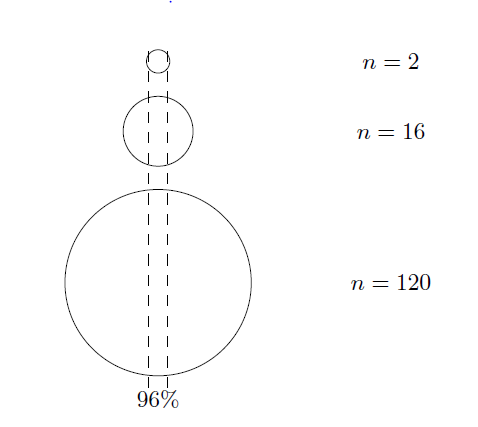
\includegraphics[width = 0.7\textwidth]{B2.png}
		\caption{96\% volume strip in different dimensions }
		\label{f:1}
	\end{figure}
	
	
	
	
	
	So volume seems to concentrate on center of ball as volume is concentrated on its  (n - 1)-dimensional slices passing through origin which are all subspace of ball and all these subspace meet on origin. But for large n as slice goes very thin and considering all such slices in each direction of ball, volume should lie near the surface of ball.\\
	
	So finally we reach to conclusion that for large dimension objects its measure(here Volume) tends to concentrate in places where our low-dimensional intution consider small.\\
	Hence our intution in lower dimension of measure distribution is wrong for higher dimension. 
	
	
	
	
	
	
	
	
	
	
	
	\subsection{Mixed Volume for Convex Body}
	\label{ss:20.5}
	First we define mixed volume for polytopes recursively:  \\
	We denote  $ \mathcal{N}(P_{1},P_{2},\ldots P_{k})$ to be the set of all facet normals of the convex polytope $P_{1}+P_{2}+ \ldots + P_{k}$
	\begin{mydef} \label{d:18}
		We define the mixed volume $V^{(n)}\left(P_{1}, \ldots, P_{n}\right)$ of $P_{1}, \ldots, P_{n}$ recursively for polytopes $P_{1}, \ldots, P_{n} \in \mathcal{P}^{n},$ 
		
		$$ \text{ for } n = 1, P_{1}=[a, b] \text { with } a \leq b,$$ 
		
		\begin{equation}
		\label{eq49}
		V^{(1)}\left(P_{1}\right):=V\left(P_{1}\right)=h_{P_{1}}(1)+h_{P_{1}}(-1) = b - a,  
		\end{equation} 
		$$\text{ and} \text { for } n \geq 2 $$ 
		\begin{equation} \label{eq50}
		\\
		V^{(n)}\left(P_{1}, \ldots, P_{n}\right):=\frac{1}{n} \sum_{u \in \mathcal{N}\left(P_{1}, \ldots, P_{n-1}\right)} h_{P_{n}}(u) V^{(n-1)}\left(P_{1}(u)\left|u^{\perp}, \ldots, P_{n-1}(u)\right| u^{\perp}\right)
		\end{equation}
	\end{mydef}     
	\begin{theorem}
		\label{t:10}
		If $\left(P_{1}^{(k)}\right)_{k \in \mathbb{N}}, \ldots,\left(P_{n}^{(k)}\right)_{k \in \mathbb{N}}$ are arbitrary approximating sequences\\
		
		converging to convex bodies  $K_{1}, \ldots, K_{n} \in \mathcal{K}^{n}$ respectively.
		\\
		i.e. each sequence of polytopes $P_{j}^{(k)}$ converges to a convex body, 
		$K_{j}, j=1, \ldots, n,$ as $k \rightarrow \infty,$ 
		then limit 
		\begin{equation}
		\label{eq51}
		V\left(K_{1}, \ldots, K_{n}\right)=\lim _{k \rightarrow \infty} V\left(P_{1}^{(k)}, \ldots, P_{n}^{(k)}\right)
		\end{equation}
		exists and does not depend on the choice of approximating sequences $\left(P_{j}^{(k)}\right)_{k \in \mathbb{N}}. $ \newline
		Mixed volume of $K_{1}, \ldots, K_{n} $ is defined to be $V\left(K_{1}, \ldots, K_{n}\right)$ \newline
		
		and the mapping $V:\left(\mathcal{K}^{n}\right)^{n} \rightarrow \mathbb{R}$ defined $b y\left(K_{1}, \ldots, K_{n}\right) \mapsto V\left(K_{1}, \ldots, K_{n}\right)$ is called mixed volume.\newline
		
		Precisely 
		\begin{equation} 
		\label{eq52}
		V\left(K_{1}, \ldots, K_{n}\right)=\frac{1}{n !} \sum_{l=1}^{n}(-1)^{n+l} \sum_{1 \leq r_{1}<\cdots<r_{l} \leq n} V\left(K_{r_{1}}+\cdots+K_{r_{l}}\right)
		\end{equation}
		and, for $m \in \mathbb{N}, K_{1}, \ldots, K_{m} \in \mathcal{K}^{n}$ and $\alpha_{1}, \ldots, \alpha_{m} \geq 0$
		
		
		\begin{equation}
		\label{eq53}
		V\left(\alpha_{1} K_{1}+\cdots+\alpha_{m} K_{m}\right)=\sum_{i_{1}=1}^{m} \cdots \sum_{i_{n}=1}^{m} \alpha_{i_{1}} \cdots \alpha_{i_{n}} V\left(K_{i_{1}}, \ldots, K_{i_{n}}\right)
		\end{equation}
	\end{theorem}
	
	\begin{properties} (\textbf{Properties of Mixed Volume for Convex Body})
		\label{prop :2}
		for all $J, K, K_{1}, \ldots, K_{n} 
		\in \mathcal{K}^{n}$ \\ 
		\begin{enumerate}
			
			\item
			$V(J, \ldots, J)=V(J)$ and $ nV(J, \ldots, J, B(1))=A(J)$ 
			
			\item 
			$V\left(K_{1}, \ldots, K_{n}\right)$ is symmetric in the indices $1,\ldots, n$
			\item
			$V$ is multilinear, i.e.
			for all $ x$,$y$ $\geq 0 $
			$$
			V\left(x J+y K, K_{2}, \ldots, K_{n}\right)=x V\left(J, K_{2}, \ldots, K_{n}\right)+y V\left(K, K_{2}, \ldots, K_{n}\right)
			$$
			\item
			for all $\alpha_{1}, \ldots, \alpha_{n} \in \mathbb{R}^{n}$
			$$
			V\left(K_{1}+\alpha_{1}, \ldots, K_{n}+\alpha_{n}\right)=V\left(K_{1}, \ldots, K_{n}\right)
			$$
			\item  
			For all rigid motions $f$ 
			$$ 
			V\left(f K_{1}, \ldots, f K_{n}\right)=V\left(K_{1}, \ldots, K_{n}\right)
			$$ 
			\item
			$V$ is continuous, i.e.
			Whenever $K_{i}^{(j)} \rightarrow K_{i}, i=1, \ldots, n$
			\[
			V\left(K_{1}^{(j)}, \ldots, K_{n}^{(j)}\right) \rightarrow V\left(K_{1}, \ldots, K_{n}\right)
			\]
			\item $V$ is positive, and in each argument,$V$ is monotone.	 
			
		\end{enumerate}
	\end{properties}
	
	\subsection{The Brunn-Minkowski Theorem}
	\label{ss:21}
	Brunn-Minkowski Theorem  basically says that the function 
	\[s  \mapsto \sqrt[n]{V(s K+(1- s) L)}, \quad s \in[0,1]
	\]
	is concave for $ K, L \in \mathcal{K}^n $.
	We will get inequalities for mixed volumes, and as a consequence also get the famous isoperimetric inequality from concavity of above function
	\\\\
	We will be using result of this following lemma further for proving Brunn-Minkowski Theorem
	\begin{lemma} 
		\label{l:2}
		For $a \in(0,1)$ and $r, s, t>0$
		\[
		\left(\frac{a}{r}+\frac{1-a}{s}\right)\left[a r^{t}+(1-a) s^{t}\right]^{\frac{1}{t}} \geq 1
		\]
		with equality, iff $r=s$
	\end{lemma} 
	\begin{proof}
		
		For proving ths result we will be using the fact that the function $x \rightarrow lnx $ is strictly concave \\
		so taking ln of the expression as argument of expression is always positive. we get 
		$$\ln \left\{\left(\frac{a}{r}+\frac{1-a}{s}\right)\left[a r^{t}+(1-a) s^{t}\right]^{\frac{1}{t}}\right\}$$
		
		$$ =\frac{1}{t} \ln \left(a r^{t}+(1-a) s^{t}\right)+\ln \left(\frac{a}{r}+\frac{1-a}{s}\right)$$
		Now using strict concavity of  function  $x \rightarrow lnx $ we get 
		$$\frac{1}{t} \ln \left(a r^{t}+(1-a) s^{t}\right)+\ln \left(\frac{a}{r}+\frac{1-a}{s}\right)
		\geq \frac{1}{t}\left(a \ln r^{t}+(1-a) \ln s^{t}\right)+a \ln \frac{1}{r}+(1-a) \ln \frac{1}{s}$$
		
		
		$$ =  \left(a \ln r+(1-a) \ln s\right)+a \ln \frac{1}{r}+(1-a) \ln \frac{1}{s}$$
		$$\quad = 0$$
		
		Now as logarithm is strict monotone function we get required result 
		\[
		\left(\frac{a}{r}+\frac{1-a}{s}\right)\left[a r^{t}+(1-a) s^{t}\right]^{\frac{1}{t}} \geq 1
		\]
		clearly equality follows when $r = s $
	\end{proof}
	
	
	
	
	
	
	
	
	
	\begin{theorem}(\textbf{Brunn-Minkowski Theorem})
		\label{t:11}
		For convex bodies $J, K \in \mathcal{K}^{n}$ and $a \in(0,1)$
		\begin{equation}
		\label{eq54}
		\sqrt[n]{V(a J+(1-a) K)} \geq a \sqrt[n]{V(J)}+(1-a) \sqrt[n]{V(K)}
		\end{equation} \label{eq:4.19}
		with equality, iff $J$ and $K$ lie in parallel hyperplanes or $J$ and $K$ are homothetic( see \ref{d:2})
	\end{theorem}
	\begin{proof}
		Based on the dimension of the convex body, we consider 4 cases.
		\hfill \break
		
		\textbf{Case 1} $: \quad \text{When } J$ and $K$ lie in parallel hyperplanes. Then  $a J+(1-) K$  also lies in a hyperplane,\quad so that $$V(J)=V(K)=0$$    $$\text{and also}$$ $$V(a J+(1-a) K)=0$$
		hence done for this case.
		\hfill \break
		\textbf{Case 2}: \quad  When $\operatorname{dim} J \leq n-1$ and $\operatorname{dim} K \leq n-1,$ but $J$ and $K$ do not lie in parallel hyperplanes, for all $a \in(0,1)$, $\operatorname{dim}(J+K)=n .$ and hence  $\operatorname{dim}(a J+(1-a) K)=n \text{ also }.$ 
		\hfill \break
		$V(J) = V(K)= 0$ as $\operatorname{dim} J,K \leq n-1 $ Therefore for all $a \in(0,1)$
		$$
		a \sqrt[n]{V(J)}+(1-a) \sqrt[n]{V(K)}=0 \leq \sqrt[n]{V(a J+(1-a) K)}
		$$
		\hfill \break
		\textbf{Case 3}: \quad  When $\operatorname{dim } J \leq n-1$ and $\operatorname{dim} K=n$ or vice versa
		\hfill \break 
		Then, for $x \in J,$ we get
		\[
		a x+(1-a) K \subset a K+(1-a) K
		\]
		and Consequently
		\[
		(1-a)^{n} V(K)=V(a x+(1-a) K) 
		\]
		as adding a point $a x $ is translation of $(1-a) K$ and won't effect Volume. 
		and
		$$ V(a x+(1-a) K) \leq V(a 
		J+(1-a) K)$$
		and equality occur, iff $J=\{x\}$ 
		\hfill \break
		\textbf{Case 4}:When $\operatorname{dim} J=\operatorname{dim} K=n .$  We are allowed to take $V(J)=V(K)=1 .$ as for general $J, K,$  we  can take
		\[
		\widetilde{J}:=\frac{1}{\sqrt[n]{V(J)}} J, \quad \widetilde{K}:=\frac{1}{\sqrt[n]{V(K)}} K
		\]
		and
		\[
		\widetilde{a}:=\frac{a \sqrt[n]{V(J)}}{a \sqrt[n]{V(J)}+(1-a) \sqrt[n]{V(K)}}
		\]
		Then we have
		\[
		\sqrt[n]{V({\widetilde{a} \widetilde{ J} }+(1-\widetilde{a}) \widetilde{K})} \geq 1
		\]
		Now  as $V(\widetilde{J}) = V(\widetilde{K})$ = 1 so $$\sqrt[n]{V(\widetilde{J})}+(1-a) \sqrt[n]{V(\widetilde {K})}=a+(1-a)=1$$
		hence $\widetilde{J}$ and $\widetilde{K}$
		follow the BRUNN-MINKOWSKI Theorem,  and also, $J$ and $K$ are homothetic, iff $\widetilde{J}$ and $\widetilde{K}$ are homothetic.Therefore,Now  we have to just prove that given condition that $V(J)=V(K)=1$, We have 
		\[
		V(a J+(1-a) K) \geq 1
		\]
		with equality iff $J, K$ are translates of each other.
		\\
		We define centre of gravity for an $n$ -dimensional convex body $S$ to be the point $c \in \mathbb{R}^{n}$ such that
		\[
		\langle c, u\rangle=\frac{1}{V(M)} \int_{S}\langle x, u\rangle d x
		\]
		for all $u \in S^{n-1} .$ 
		By translating  $J$ and $K$ we can have their centre of gravity at 0 as the Volume is translation invariant,the equality case then just reduces to claim hat $K=L$
		\hfill \break
		Now by induction on $n$, We prove  BRUNN-MINKOWSKI Theorem 
		\hfill \break
		For $n=1$, 1 - dimensional volume is linear so Brunn-Minkowski inequality easily follows   
		\hfill \break 
		Along with above conclusion we also get that equality corresponds to the fact that two convex bodies (which are compact intervals in $\mathbb{R}$), in $\mathbb{R}$  are homothetic.
		\hfill \break 
		Now for $n \geq 2$ if the Brunn-Minkowski theorem is true in dimension $n-1 $
		\\
		we choose a unit vector $u \in S^{n-1}$ and denote 
		the hyperplane $E_{\lambda}$ in the direction $u$ with  distance(signed) $\lambda \in \mathbb{R} $ from the origin defined by 
		\[
		E_{\lambda}:=\{x:\langle\ x, u\rangle=\lambda\}, 
		\]
		Now since by Fubini's theorem  
		\[
		V(K \cap\{x: \langle x, u\rangle \leq \beta\}) = \int_{-h_{ K(-u)}}^{\beta} v\left(K \cap E_{\lambda}\right) d \lambda
		\] 
		The function
		\[
		g:\left[-h_{K}(-u), h_{K}(u)\right] \rightarrow[0,1], \quad \gamma \mapsto V(K \cap\{x:\langle x, u\rangle \leq  \gamma \}
		\]
		would be  continuous and strictly increasing\\
		where $-h_{K}(-u), h_{K}(u)$ are support function of K at $u$ and $-u$ and are extreme upper point and extreme lower point respectively.
		\hfill \break
		Map $\lambda \mapsto v\left(K \cap E_{\lambda}\right)$ is continuous on $\left(-h_{K}(-u), h_{K}(u)\right),$ where $v$ is area functional.
		%some doubt in v is  area measure 
		$g$ is differentiable function on $\left(-h_{K}(-u), h_{K}(u)\right)$ and $$g^{\prime}(\beta)=v\left(K \cap E_{\beta}\right)$$
		\\
		since $g$ is invertible, inverse function of $g$, $ \gamma:[0,1] \rightarrow\left[-h_{K}(-u), h_{K}(u)\right],$ which is also a continuous function and strictly increasing  function satisfies $ \gamma(0)=-h_{K}(-u),  \gamma(1)=h_{K}(u)$ and
		\[
		\gamma^{\prime}(\tau)=\frac{1}{g^{\prime}( \gamma(\tau))}=\frac{1}{v\left(K \cap E_{ \gamma(\tau)}\right)}, \quad  \text{where } \tau \in(0,1)
		\]
		Similarly, For K
		The function
		\[
		f:\left[-h_{K}(-u), h_{K}(u)\right] \rightarrow[0,1], \quad \delta \mapsto V(K \cap\{x:\langle x, u\rangle \leq  \delta \}
		\]
		and in the same way
		we get its inverse function $ \delta:[0,1] \rightarrow\left[-h_{L}(-u), h_{L}(u)\right]$     with 
		\[
		\delta^{\prime}(\tau)=\frac{1}{v\left(L \cap E_{\delta(\tau)}\right)}, \quad  \text{where } \tau \in(0,1)
		\]
		Because of
		\[
		a\left(K \cap E_{g(\tau)}\right)+(1-a)\left(L \cap E_{\delta(\tau)}\right) \subset(a K+(1-a) L) \cap E_{a \gamma(\tau)+(1-a) \delta(\tau)}
		\]
		for $a, \tau \in[0,1],$ we obtain from the inductive assumption
		\[
		\begin{array}{l}
		V(a J+(1-a) K) \\\\
		\quad=\int_{-\infty}^{\infty} v\left((a J+(1-a) K) \cap E_{\lambda}\right) d \lambda \\\\
		\quad=\int_{0}^{1} v\left((a J+(1-a) K) \cap E_{a \gamma(\tau)+(1-a) \delta(\tau)}\right) \\\\
		\quad  \quad \quad \quad \quad \quad \quad \quad \quad \times
		\left(a \gamma^{\prime}(\tau)+(1-a) (\delta)^{\prime}(\tau)\right) d \tau
		\\\\\\
		\geq \int_{0}^{1} v\left(a\left(J \cap E_{\gamma(\tau)}\right)+(1-a)\left(K \cap E_{\delta(\tau)}\right)\right)
		\\\\
		\quad \quad \quad \quad \quad \quad \quad \quad \quad \quad \quad
		
		\times
		
		\left\{\frac{a}{v\left(J \cap E_{\gamma(\tau)}\right)}+\frac{1-a}{v\left(K \cap E_{\delta(\tau)}\right)}\right\} d \tau \\\\\\
		\geq \int_{0}^{1} \left\{  a^{n-1} \sqrt{v\left(K \cap E_{\gamma(\tau)}\right)}+(1-a) \sqrt[n-1]{v\left(L \cap E_{\delta(\tau)}\right)} \right\}^{n-1} \\\\
		\quad \quad \quad \quad \quad \quad \quad \quad \quad \quad \quad \times \left\{ \frac{a}{v\left(J \cap E_{\gamma(\tau)}\right)}+\frac{1-a}{v\left(K \cap E_{\delta(\tau)}\right)}\right\} d \tau
		\end{array}
		\]
		Choosing $r:=v\left(J \cap E_{\gamma(\tau)}\right), s:=v\left(K \cap E_{\delta(\tau)}\right)$ and $t:=\frac{1}{n-1},$
		\\
		applying  Lemma \ref{l:2} on above expression written inside integration is $\geq 1,$ and on the limi of 0 and 1 whole integrand also get  $\geq 1,$ which gives the required result.
		\\
		Now For equality case assume that equality occur so that
		\[
		V(a J+(1-a) K) = 1 
		\]
		For above expression equal to $1,$ in our last estimation we must have equality, which means that the integrand  is equal to $1,$ for all $\tau .
		$ and this the equality case(iff $r = s$) of same Lemma \ref{l:2}
		\\
		So we have 
		\[
		v\left(J \cap                E_{\gamma(\tau)}\right)=v\left(K \cap E_{\delta(\tau)}\right), \quad \text { for all } \tau \in[0,1]
		\]
		Hence $g^{\prime}= \delta^{\prime},$ so $\gamma- \delta$ is a constant.\\
		Because the centre of gravity of $J$ is at the origin, we get 
		\\
		\[
		0=\int_{J}\langle x, u\rangle d x=\int_{\gamma(0)}^{\gamma(1)} \lambda v\left(K \cap E_{\lambda}\right) d \lambda=\int_{\gamma(0)}^{\gamma(1)} \lambda \gamma^{\prime}(\lambda) d \lambda=\int_{0}^{1} \gamma(\tau) d \tau
		\]
		where the change of variables $\lambda=\gamma(\tau)$ was used. In an analogous way,
		\[
		0=\int_{0}^{1} \delta(\tau) d \tau
		\]
		Consequently,
		\[
		\int_{0}^{1}(\gamma(\tau)-\delta(\tau)) d \tau=0
		\]
		and therefore $\gamma=\delta .$ In particular, we obtain
		\[
		h_{J}(u)=\delta(1)=\delta(1)=h_{K}(u)
		\]
		since $u$ was arbitrary, $V(a J+(1-a) K)=1$ implies $h_{J}=h_{K},$ and hence $J=K$ \\
		Conversely,when $J=K$ 
		$$V(a J+(1-a) K)=V(a J+(1-a) J) =  V(J) = 1 $$
		Hence Proved
	\end{proof}
	%change to modify language please looks like totally book
	\hfill \break
	
	\begin{corollary}
		
		function $ S(b):b\rightarrow \sqrt[n]{V(bJ+(1-b)K)}$  is concave on $[0,1] .$ 
	\end{corollary}
	\begin{proof}
		
		\[
		S(b):=\sqrt[n]{V(b J+(1-b) K)}
		\] 
		is  easily using above theorem \ref{t:11}
		\hfill \break
		we have to prove that 
		$$ S(a x+(1-a) y) \geq a S(x)+(1-a) S(y) $$
		
		Let $x, y, a \in[0,1],$ 
		
		\hfill \break
		
		$  S(ax+(1-a)y)  =\sqrt[n]{V([ax+(1-a)y] J+[1-a x-(1-a) y] K)}$
		
		\hfill \break
		
		\quad \quad \quad \quad \quad \quad \quad \quad 
		$=\sqrt[n]{V(a[x J+(1-x) K]+(1-a)[y J+(1-y) K])}$
		
		\hfill \break
		
		\quad \quad \quad \quad \quad \quad \quad \quad   $
		\geq a \sqrt[n]{V(x J+(1-x) K)}+(1-a) \sqrt[n]{V(y J+(1-y) K)}
		\quad \quad \quad \quad \quad \text{from Theorem } \ref{t:11}$
		
		\hfill \break
		
		$ \quad \quad \quad \quad \quad  \quad  \quad \quad = a S(x)+(1-a) S(y)$
	\end{proof}
	
	
	
	
	
	
	
	
	
	
	
	
	
	
	\begin{theorem}
		\label{t:12}
		For $J, K \in \mathcal{K}^{n}$
		\[
		V(J, \ldots, J, K)^{n} \geq V(J)^{n-1} V(K)
		\]
		with equality, if and only if $\operatorname{dim} J \leq n-2$ or $J$ and $K$ lie in parallel hyperplanes or $J$ and $K$ are homothetic.
		\\
	\end{theorem} 
	Now as a corollary of above theorem we get famous Isoperimtric Inequality for convex body 
	which states that, 
	
	\hfill \break
	
	Between all convex bodies of given volume, the balls have the smallest surface area given surface area. 
	
	\quad\quad\quad\quad\quad\quad\quad\quad\quad\quad\quad\quad\quad\quad
	or 
	\hfill \break
	Between all convex bodies of given surface area, the balls have the largest volume.
	
	\hfill \break
	%may add if proof is clear to you 
	% \begin{proof}
	
	
	%  For $\operatorname{dim} K \leq n-1$, the inequality holds since the right-hand side is zero. Moreover, we then have equality, if and only if either $\operatorname{dim} K \leq n-2$ or $K$ and $L$ lie in parallel hyperplanes (compare Exercise 3.3 .1 ). Hence, we now assume $\operatorname{dim} K=n$ By Theorem 3.4 .2 (similarly to the preceding remark), it follows that the function
	% \[
	% f(t):=V(K+t L)^{\frac{1}{n}}, \quad t \in[0,1]
	% \]
	% is concave. Therefore
	% \[
	% f^{+}(0) \geq f(1)-f(0)=V(K+L)^{\frac{1}{n}}-V(K)^{\frac{1}{n}}
	% \]
	% since
	% \[
	% f^{+}(0)=\frac{1}{n} V(K)^{\frac{1}{n}-1} \cdot n V(K, \ldots, K, L)
	% \]
	% we arrive at
	% \[
	% V(K)^{\frac{1}{n}-1} \cdot n V(K, \ldots, K, L) \geq V(K+L)^{\frac{1}{n}}-V(K)^{\frac{1}{n}} \geq V(L)^{\frac{1}{n}}
	% \]
	% where we used the Brunn-Minkowski inequality in the end (with $t=\frac{1}{2}$ ). This implies the assertion. Equality holds if and only if equality holds in the Brunn-Minkowski inequality, which yields that $K$ and $L$ are homothetic.      
	%  \end{proof}     
	
	
	
	
	
	
	
	
	
	
	\begin{corollary}\textbf{(Isoperimetric Inequality for Convex Body)}       
		
		
		Assume that $K \in \mathcal{K}^{n}$ is a convex body of dimension $n .$ Then,
		
		$$\frac{{A(K)}^n}{{V(K)}^{n-1}} \geq \frac{{A(B(1))}^{n}}{{V(B(1))}^{n-1}} $$
		
		with equality  iff  $K$ is a ball.
		
	\end{corollary}
	\begin{proof}
		
		
		On putting $K:=B(1)$ in Theorem \ref{t:12} we get 
		\[
		V(K, \ldots, K, B(1))^{n} \geq V(K)^{n-1} V(B(1))
		\]
		as $$V(B(1), \ldots, B(1), B(1)) = V(B(1))$$ from properties(\ref{prop :2}) of mixed volume \\
		
		We can write it in other form
		\[
		\frac{n^{n} V(K, \ldots, K, B(1))^{n}}{n^{n} V(B(1), \ldots, B(1), B(1))^{n}} \geq \frac{V(K)^{n-1}}{V(B(1))^{n-1}}
		\]
		
		Now using  properties (\ref{prop :2}) of mixed volume we have
		
		$$ nV(K, ..., K, B(1)) = A(K),\quad  \quad \quad nV(K, ..., K, B(1)) = A(K) $$ 
		So
		We get \[
		\left(\frac{A(K)}{A(B(1))}\right)^{n} \geq\left(\frac{V(K)}{V(B(1))}\right)^{n-1}
		\]
		And then finally get required Isoperimetric Inequality
	\end{proof}
	
	As we know volume and area of $B(1)$, 
	$$V(B(1))=\kappa_{n} \text{  \quad \quad and \quad \quad   } A(B(1))=n \kappa_{n},$$
	we can re-write it  in terms of $\kappa_{n}$
	
	\[
	V(K)^{n-1} \leq \frac{1}{n^{n} \kappa_{n}} A(K)^{n}
	\]
	\hfill \break
	
	From here for $\mathbb{R}^{2}$ plane, i.e. $n=2$ we get Isoperimetric Inequality  
	\[
	A(K) \leq \frac{1}{4 \pi} L(K)^{2}
	\]
	Where  $A(K)$ is usual  area ( volume in $\mathbb{R}^{2}$ ) and $L(K)$ is the boundary length \newline  ( surface area in $\mathbb{R}^{2}$ ), \\
	
	Similarly  for $n=3$
	we get
	
	\[
	V(K)^{2} \leq \frac{1}{36 \pi} A(K)^{3}
	\]
	
	
	



	
	
	
	
	
	
	\chapter{Isoperimetric Inequaity for Graph}
	\section{Introduction}
	\label{s:5}
	
	Isoperimetric Inequality for a Graph G is defined in similar way as defined in $\mathbb{R}^n$. it involves finding a subset of the Vertex set V(G) of G among all subsets of fixed size, which has the smallest edge-boundary. These subsets are called Isoperimetric Sets. Further  Isoperimetric Sets are given for some trivial and non-trivial classes of Graph. \par 
	From paper [\ref{bib:4}], Isoperimetric number $i(G)$ and $i_k{G}$ are defined, and some basic properties of $i(G)$  are discussed. Then the main theorem for this project is proved from section 6 which uses theorem from section 4 regarding lower bound for $i_k{G}$ and for i(G) in terms of the second eigenvalue of difference Laplacian matrix D and uses theorem regarding bounding expectation of the second eigenvalue of random 2k-regular Graph from different paper [\ref{bib:5}]. For proof of this theorem from [\ref{bib:5}], some results are used without proof from paper [\ref{bib:6}] and [\ref{bib:7}].
	
	\hfill \break
	
	
	\subsection{Isoperimetric Inequality for Graph G}
	For a graph G with vertex set V and edge set E, Isoperimetric Inequality is to find a function $\mathcal{F}$, called best  Isoperimetric function such that  \begin{center}
		$|\partial \Omega| \geq \mathcal{F}(|\Omega|)$  
	\end{center}   
	for every non empty subset $\Omega$ of vertices set V, where $\partial \Omega$ is the boundary of $\Omega$  and defined as the set of edges of the graph connecting vertices of $\Omega$ with vertices of its complement $\bar{\Omega} = V \backslash \Omega $ and $\mathcal{F}$ is defined as  \begin{center}
		$\mathscr{F}(k)=\min _{|\Omega|=k}|\partial \Omega|$\par
	\end{center} 
	Best Isoperimetric function or corresponding Sharp Isoperimetric Inequality is known only for few classes of graph e.g.
	from combinatorial arguments 
	\par
	\begin{itemize}
		\item For The complete graph $K_{n}$ inequality is $|\partial \Omega|=(n-|\Omega|) | \Omega|$ 
		\item For The cycle $C_{n}$ it is  $|\partial \Omega|\geq 2$ for $|\Omega| \neq n$.
		\item For The infinite d-regular tree it is $|\partial \Omega| \geq(d-2)| \Omega|+2$\par
	\end{itemize}
	
	
	
	Other Non-trivial classes for which it is known are some families of cartesian products of graphs. like 
	n-cube $Q_{n}$, 
	grid $[k]^{n}$,
	and lattice $\mathbb{Z}^{n}$.
	\par
	Apart from these combinatorial techniques There are eigenvalue techniques which give good Isoperimetric Inequality in general \\\\
	
	Using eigenvalue techniques, 
	Isoperimetric Inequality for d-regular Graph in terms of second eigenvalue $\lambda_2$\ is following. \par
	
	Let $\lambda_{2}$ be the second smallest eigenvalue of Laplacian L of G then for a random d-regular graph $|\partial \Omega| \geq \lambda_{2} \frac{|\Omega||\bar{\Omega}|}{|V|}$  is a good approximation of best Isoperimetric function from the work of Friedman and Bollobas  \par 
	
	
	{Laplacian matrix L of G }
	\label{ss:22}
	Laplacian matrix L of G is defined as  $L = D - A$ where  D be n x n diagonal matrix $D_{jj} = d_{j}$ and A is adjacency matrix of the Graph G.\par
	
	
	
	It is clear that   $L_{ij} = -1$ for $i\neq j$  for $ij\in E(G)$,  $L_{ii}$ = $d_i$(degree of ith vertex) and   $L_{ij} = 0$ otherwise.\par
	
	It can be easily seen that L is asymmetric and a positive definite  matrix so its eigenvalues are real and positive. \\
	
	Let $\mu_{1} \leq \mu_{2} \leq \cdots \leq \mu_{n}$, $\mu_{i} \geq 0$  be  eigenvalues of L then smallest eigen value $\mu_{1} = 0$ as row sum of L  be 0 and all-ones vector(each entry is 1) is an eigen vector of eigen value 0. That's why we consider second smallest eigen value of L. Largest eigen value of Adjacency Matrix is found to be d for regular-d Graph. \par
	
	
	
	
	In general, there is no simple relationship between the eigenvalues of
	A and the eigenvalues of L but In case of d-regular graphs, d is the
	common vertex degree and $L = dI - A$  so if $\lambda_{1} \geq \lambda_{2}....\geq \lambda_{n}$  be the eigenvalues of A, we have eigenvalues of L are $\mu_{j} = d - \lambda_{j}$ (each eigenvalue of sum of two matrix is sum of corresponding  individual eigenvalue if both matrix commute multiplicatively). \\\\
	Throughout the report, We will denote $\lambda_{2} $ to be a second largest eigenvalue of the adjacency matrix A and $\mu_{2}$ to be the second smallest eigenvalue of corresponding Laplacian matrix of A for 2k-regular Graph.  
	
	
	
	\subsection{Isoperimetric Number of Graph G} \label{ss:23}
	
	
	The Isoperimetric number of Graph G is defined as \par
	\begin{center}
		$i(G)=\min _{\Omega} \frac{|\partial \Omega|}{|\Omega|}$
	\end{center}
	where minimum is taken over all nonempty subsets $\Omega$ of V satisfying\par $|X| \leq \frac{1}{2}|V(G)|$.
	\\           We can think of the quantity  $\frac{|\partial \Omega|}{|\Omega|}$ as the average boundary degree of X. \par
	i(G) can also be defined in following way \par
	\begin{center}
		$i(G)=\min \frac{|E(X, Y)|}{\min \{|X|,|Y|\}}$
	\end{center}
	where minimum runs over all partitions of V into nonempty subsets X and Y such that  $V=X \cup Y$ and $E(X, Y)=\partial X=\partial Y$ are the edges between X and Y.
	\par
	The isoperimetric constant can be understood as a measure of how easy
	it is to disconnect a large part of the graph. \par
	For getting i(G) we have to find small edge-cut $E(X, Y)$ separating as large as possible  subset X from the remaining larger part Y assuming $|X|\leq |Y|$ so in this way i(G) can serve as measure of connectivity of Graph. \\\\
	Some results for different classes of Graphs are following \par
	\begin{enumerate}
		
		
		\item  $i(G)=0$ if and only if $G$ is disconnected \par
		Proof. we can choose  any part of the graph which is not connected to rest of Graph and will get $i(G)=0$ \par
		\item  If $G$ is $k$ -edge-connected(require at least k edge to break connectivity) then $i(G) \geq 2 k /|V(G)|$ \par
		Proof. For any chosen subset X of V,we have  $|\partial X| \geq k$ and we can take $|X|$ to be $|V(G)|/2$ and hence done\par
		\item  If $\delta$ is the minimal degree of vertices in $G$ then $i(G) \leq\delta$ \par
		\item  If   $e=u v$ is   an  edge  of G  and $|V(G)| \geq 4$ \par then  $i(G) \leq [deg(u)+deg(v)-2] / 2$ \par
	\end{enumerate}
	
	
	
	
	Isoperimetric number for some classes of Graph are following \par
	\begin{enumerate}
		\item   For the complete graph $K_{n}, i\left(K_{n}\right)=\lceil n / 2\rceil$ \par
		\item The cycle $C_{n}$ has $i\left(C_{n}\right)=2 /\lfloor n / 2\rfloor$ \par
		\item  The path $P_{n}$ on $n$ vertices has $i\left(P_{n}\right)=1 /\lfloor n / 2\rfloor$
	\end{enumerate}
	\section{Bounding $\mathrm{E}\left|\lambda_{2}(G)\right|$ of random 2d-regular Graph}
	\label{s:6 }
	Here  we will be con
	
	
	\begin{theorem} \label{t:13}
		$ \left(\mathbf{A} \right) $ For $G \in{G}_{n, 2d}$ we have
		$$
		\mathbf{E}\left|\lambda_{2}(G)\right| \leq 2 \sqrt{2 d-1}\left(1+\frac{\log d}{\sqrt{2 d}}+o\left(\frac{1}{\sqrt{d}}\right)\right)+O\left(\frac{d^{3 / 2} \log \log n}{\log n}\right)
		$$  and we have \begin{center}
			$\mathrm{E|\lambda_{2}(G)|} \leq O(d^{1/2})$ when d is fixed and $n\rightarrow \infty$
		\end{center}
		where E denotes the expected
		value over ${G}_{n, 2d}$      and more generally we have\\\\ $\mathbf{E}\left|\lambda_{2}(G)\right|^{m} \leq\left(2 \sqrt{2 d-1}\left(1+\frac{\log d}{\sqrt{2 d}}+O\left(\frac{1}{\sqrt{d}}\right)\right)+O\left(\frac{d^{3 / 2} \log \log n}{\log n}\right)\right)^{m}$ \par
		for any $ m \leq 2\lfloor\log n\lfloor\sqrt{2 d-1} / 2\rfloor / \log d\rfloor$\\\\
		$ \left(\mathbf{B}\right) $   As a corollary, For a $\beta\geq 1$ we have \par
		$\left|\lambda_{2}(G)\right| \geq\left(2 \sqrt{2 d-1}\left(1+\frac{\log d}{\sqrt{2 d}}+O\left(\frac{1}{\sqrt{d}}\right)\right)+O\left(\frac{d^{3 / 2} \log \log n}{\log n}\right)\right) \beta$\\\\
		with probability
		$$
		\leq \frac{\beta^{2}}{n^{2}\lfloor\sqrt{2 d-1} / 2\rfloor \log \beta / \log d}
		$$   \\\\
	\end{theorem}
	\begin{proof}
		The standard approach to estimating eigenvalues is to estimate the trace of high power of the adjacency matrix.\par
		First we define ${G}_{n, 2d}$, probability space of 2d-regular Graphs on n vertices    we choose d permutation of the numbers ${1,\ldots n}$ each permutation equally likely and construct a direct Graph $G = (V,E) $ with  vertex set $V=\{1, \ldots, n\}$ and edges\par
		$E=\left\{\left(i, \pi_{j}(i)\right),\left(i, \pi_{j}^{-1}(i)\right) | j=1, \ldots, d \quad i=1, \ldots, n\right\}$ \\\\
		Constructed graph G will have possibly multiple edges and self-loops, and which is symmetric in the sense that for every edge in the Graph, the opposite edge is also there. Although G is directed, we can view it as an undirected graph by
		replacing each pair of edges $(i, \pi(i)), (\pi(i), i) $ with one undirected edge.\par In this way, Each vertex of this Graph has its degree 2d, and  We denote
		this probability space of random graphs by $G_{n,2d}$. \\\\
		Let $A$ be the adjacency matrix of a graph $G \in \mathscr{G}_{n, 2 d}$. Let $\Pi$ be the alphabet of symbols
		$$
		\Pi=\left\{\pi_{1}, \pi_{1}^{-1}, \pi_{2}, \ldots, \pi_{d}^{-1}\right\}
		$$
		where  $\pi_{1}, \ldots, \pi_{d}$ are  $d$ permutations from which $G$ was constructed, and any word, $w=\sigma_{1} \ldots \sigma_{k}$ of $\Pi^{*}$ as the permutation which is the composition of the permutations $\sigma_{1}, \ldots, \sigma_{k} .$ \par
		Define  \begin{center}
			$i \stackrel{w}{\rightarrow} j \equiv\left\{\begin{array}{ll}
			1 & \text { if  }  w(i)=j \\
			0 & \text { otherwise }
			\end{array}\right\}$ 
		\end{center}
		Then  $i, j$ -th entry of $A^{k}$ will be 
		$$
		\sum_{w \in \Pi^{k}} i \stackrel{w}{\rightarrow} j
		$$
		What we want is  to estimate expectation of  trace, so we need to take the expectation of the above sum only for  $i = j$      
		In evaluating $i \stackrel{w}{\rightarrow} i,$  $\pi \pi^{-1}$ with $\pi \in \Pi $    will fix the vertex so we can cancel this type of pairs in  $w$.\par
		We define a word $w \in \Pi^{k}$ to be irreducible if $w$ has no pair of consecutive letters of the form $\pi \pi^{-1}$ and denote the set of irreducible words of length $k$ by Irred $_{k} .$\par
		For 1st position of a word, first letter has  2d choices and then its next letter can not be its inverse so all other k - 1 letters will have only 2d - 1 choices so
		Irred $_{k}$ has its  size $2 d(2 d-1)^{k-1} .$ \par 
		It turns out that to estimate the second eigenvalue it suffices
		to get an estimate of the form
		$$
		\sum_{\boldsymbol{w} \in \text { Irred }_{\boldsymbol{k}}} i \stackrel{w}{\rightarrow} i=2 d(2 d-1)^{k-1} \frac{1}{n} + error 
		$$
		for all fixed i with some small error term which will be bounded later.\par
		1/n comes because we expect  that words in $Irred_{k} $ send a fixed vertex to each  others with more or less equal probability which is 1/n . \\\\
		We have following result as a corollary and will be using this result to estimate the expected sum of the k-th powers of the eigenvalues \par
		\text { For any fixed } i, $k \geq 1$, \text { and } $d-2>\sqrt{2 d-1} / 2$ \text { (i.e. } $d \geq 4)$ we have
		$$
		\mathrm{E}\left\{\sum_{w \in \mathrm{Irred}_{k}} i \stackrel{w}{\rightarrow} i\right\}=2 d(2 d-1)^{k-1}\left(\frac{1}{n}+\operatorname{error}_{n, k}\right)
		$$
		where
		$$
		\operatorname{error}_{n, k} \leq(c k d)^{c}\left(\frac{k^{2 \sqrt{2 d}}}{\left.n^{1+\lfloor\sqrt{2 d-1} / 2}\right\rfloor}+\frac{(2 d-1)^{-k / 2}}{n}\right)
		$$
		All words in $\Pi^{k}$ can be reduced to irreducible words by removing occurrences of $\pi \pi^{-1}$ in the word, and this irreducible word is independent of how the reducing was done. \par 
		Let  $p_{k,s}$ is the probability that a random word in  $\Pi^{k}$ reduces to an irreducible word of size s then breaking sum over words in  $\Pi_k$ to sum over irreducible words of size s  we get  
		$$
		\frac{1}{(2 d)^{k}} \mathbf{E}\left\{\sum_{w \in \Pi^{k}} i\rightarrow i\right\}=p_{k, 0}+\sum_{s=1}^{k} p_{k, s} \frac{1}{2 d(2 d-1)^{s-1}} \mathrm{E}\left\{\sum_{w \in \mathrm{Irred}_{s}} i \stackrel{w}{\rightarrow} i\right\}
		$$
		since $\sum_{s} p_{k, s}=1,$ we have
		$$ 
		\frac{1}{(2 d)^{k}} \sum_{i} \mathrm{E}\left\{\sum_{w \in \Pi^{k}} i \stackrel{w}{\rightarrow} i\right\}=1+(n-1) p_{k, 0}+\sum_{s=1}^{k} n p_{k, s} \operatorname{error}_{n, s} 
		$$    ..........(1)\par
		We are using following result for $p_{2k},{2s}$ without proof( proof is in paper [3])  \par
		$$
		p_{2 k, 2 s} \leq \frac{2 s+1}{2 k+1}\left(\begin{array}{c}
		2 k+1 \\
		k-s
		\end{array}\right)\left(\frac{1}{2 d}\right)^{k-s}\left(1-\frac{1}{2 d}\right)^{2 s-1}
		$$
		Note that k and s can not have different parity as  $\pi$ and $\pi^{-1}$ will get vanish in pair\par
		from proof of above from [3] it is seen that(Using here as a result)  
		$$ p_{2 k, 0} \geq \frac{1}{2 k+1}\left(\begin{array}{c}
		2 k+1 \\
		k
		\end{array}\right) \frac{(2 d-1)^{k}}{(2 d)^{2 k}}$$
		It follows that for any graph of degree $2 d$,
		$$
		\sum_{i=1}^{n} \lambda_{i}^{2 k} \geq(2 d)^{2 k}(n-1) p_{k, 0} \approx(n-1) 2^{2 k}(2 d-1)^{k}
		$$
		so that taking $2 k$ slightly less than $2 \log _{d} n$ results 
		$$
		\left|\lambda_{2}\right| \geq 2 \sqrt{2 d-1}+O\left(\frac{1}{\log _{d} n}\right)
		$$
		Now we take $k=2$ $\lfloor\log n\lfloor\sqrt{2 d-1} / 2\rfloor / \log d\rfloor,$ so that $k$ is even, and calculate
		using the simplified bound
		$$
		p_{2 k, 2 s} \leq 2^{2 k}\left(\frac{1}{2 d}\right)^{k-s}
		$$
		It is easy to see that the dominant terms of the summation over $s$ in equation (1) are $s=1$ and $s=k,$ and therefore
		$$
		\mathrm{E}\left\{\sum_{i=2}^{n} \lambda_{i}^{k}\right\} \leq n^{1+\frac{\log 2}{\log \alpha}(c k d)^{c} k^{2 \sqrt{2 d}}(2 \sqrt{2 d} \sqrt{\frac{2 d}{2 d-1}})^{k}}
		$$
		Taking $k$ -th roots, applying Hölder's  inequality, and noticing that
		$$
		\left(n^{1+\frac{\log 2}{\log d}}\right)^{1 / k}=1+\frac{\log d}{\sqrt{2} \bar{d}}+O\left(\frac{1}{\sqrt{d}}\right)
		$$
		and 
		$$
		(c k d)^{c / k} k^{2 \sqrt{2 d} / k}=1+O\left(\frac{\log d \log \log n}{\log n}\right)
		$$
		and that
		$$
		k \leq \frac{1}{c d^{3 / 2}} n^{\frac{1}{c \sqrt{a}}}
		$$
		for
		$$
		\frac{\log n}{\log \log n} \geq c^{\prime} \sqrt{d}
		$$
		proves Theorem(A)  \par 
		From here it is clear that $\mathrm{E|\lambda_{2}(G)|} \leq O(d^{1/2})$ as $\frac{ \log \log n}{\log n}\rightarrow 0$ in limit  as n goes to  infinity 
	\end{proof} 
	\begin{theorem} 
		\label{t:14}
		Let $G$ be a graph on $n$ vertices and let $\mu_{2}$ be the second smallest eigenvalue of its difference Laplacian matrix D. Then for every k, 
		$1 \leq k \leq n-1$
		$$
		i_{k}(G) \geq \frac{(n-k) \mu_{2}}{n}
		$$
		and, consequently, $i(G) \geq \mu_{2} / 2$ \par
	\end{theorem} 
	\begin{proof}
		for the second smallest eigenvalue $\mu_{2}$ of $D$ and for an arbitrary $X \subseteq V(G)$ the following relation holds(from paper [4]):
		$$
		\mu_{2} \leq|\partial X|\left(\frac{1}{|X|}+\frac{1}{|V \backslash X|}\right)
		$$
		putting $|X| = k $ and $|V\backslash X| = n-k $ and using definition of $i_k(G)$ 
		$ \mu_{2} \leq|\partial X|\left(\frac{1}{k}+\frac{1}{n-k}\right)$ = $|\partial X|\left(\frac{n}{k(n-k)}\right) $ \par
		which gives required result\\\\
	\end{proof} 
	
	\begin{mydef} \label{d:19}
		
		
		$F(n, k)$:= max$\left\{i(G)| \textit{G is k-regular  n vertices} \right\}$ 
		and
		$$
		f(k):=\lim _{n \rightarrow \infty} \sup F(n, k)
		$$
	\end{mydef}
	
	
	\begin{theorem}
		\label{t:15}
		
		
		$$f(2 k) \geq k-O\left(k^{1 / 2}\right)$$ 
		
	\end{theorem}
	
	
	\begin{proof} 
		From theorem 5.1, we have  $\mathrm{E|\lambda_{2}(G)|}
		\leq O(k^{1/2})$ when d is fixed and $n\rightarrow \infty$ for second largest eigen value $\lambda_{2}$ of Adjacency Matrix A, so second smallest eigen value($\mu_{2}$ of corresponding laplacian Matrix (or second eigen value of L) will be $2k - \lambda_{2}$ \\
		
		
		As $f(k)$ is limsup of $F(n,k)$s and each $F(n,k)$ is maximum over $i(G)$ of k-regular graphs G
		so $i(G)\leq f(2k)$
		
		From Theorem 5.2 we have
		
		$$i(G) \geq \frac{\mu_2}{2} = \frac{2k - \lambda_{2}}{2}  $$
		
		So we have
		
		$$
		f(2k) \geq \frac{2k - \lambda_{2}}{2}
		$$
		
		If we take expectation over $\mathscr{G}_{n, 2 d}$ on both side we get 
		$$
		f(2k) \geq \frac{2k - E(\lambda_{2})}{2}
		$$
		and as $\mathrm{E|\lambda_{2}(G)|}
		\leq O(k^{1/2})$ we have 
		$$
		f(2k) \geq \frac{2k - O(k^{1/2})}{2} \geq k - O(k^{1/2}) 
		$$
		
	\end{proof}  
	
	
	\addcontentsline{toc}{chapter}{Bibliography}
	\begin{thebibliography}{300}
		\bibitem{a} \label{bib:1} 
		Wolfgang Weil: A Course
		on
		Convex Geometry
		\bibitem{b} \label{bib:2}
		Issac Chavel: Isoperimetric Inequalities (Differetial Geometric and Analytic Perspective)
		\bibitem{3}     \label{bib:3}
		Keith Ball:An Elementry Introduction to Modern Convex Geometry
		University of Karlsruhe
		2002/2003
		revised version 2004/2005
		
		\bibitem{4}    \label{bib:4}
		BOJAN MOHAR: Isoperimetric numbers of Graph.
		
		
		
		\bibitem{5} \label{bib:5}
		JOEL FRIEDMAN: On the Second Eigenvalue and Random Walks in Random d-regular Graphs.
		\bibitem{6}    \label{bib:6}
		
		ANDREI BRODER, and ELI SHAMIR: On the second eigenvalue of random regular graphs. In 28th annual Symposium on Foundations of Computer Science, pages 286-294, 1987. 
		
		\bibitem{spherical_psf}      \label{bib:7}
		N.ALON and V.D. MILMAN,$\lambda_{1}$ isoperimetric inequalities for graphs, and super concentrator, J Combin Theory Ser.B38(1985),73-88  
	\end{thebibliography}  
	
	
	
	
	
	
	
	
	
	
	
	
	
	
	
	
	
	
	
	
	
	
	
	
	
	
	
	
	
	
	
	
	
	
	
	
	
	
	
	
	
	
	
	
	
	
	
	
	
	
	
	
	
	
	
	
	
	
	
	
	
	
	
	
	
	
	
	
	
	
	
	
	
	
	
	
	
	
	
	
	
	
\end{document}
